% !TeX spellcheck = de_DE
\documentclass[
	oneside,  % falls doppelseitiger Druck gewünscht, "oneside" durch "twoside" ersetzen
	ngerman, 
	final, 
	11pt, 
	a4paper, 
	1.1headlines, 
	headinclude=false, 
	footinclude=false, 
	mpinclude=false, 
	pagesize, 
	onecolumn, 
	titlepage, 
	parskip=half, 
	headsepline, 
	chapterprefix=false, 
	version=first, 
	listof=totoc, 
	bibliography=totoc, 
	toc=graduated, 
	fleqn
]{scrbook}

%%%%%%%%%%% Verwendete Pakete %%%%%%%%%%%
\usepackage[T1]{fontenc}
\usepackage[utf8]{inputenc}
\usepackage{babel}
\usepackage{hyperref}
\hypersetup{
	colorlinks=true,
	linkcolor=black,
	urlcolor=black,
	linktoc=all,
	citecolor=black
}
\usepackage{float}
\usepackage{graphicx}
\usepackage{textpos} 
\usepackage{tocloft}
\usepackage{lipsum}
\usepackage{color}
\usepackage[onehalfspacing]{setspace}
\usepackage{acronym}
\usepackage{multicol}
\usepackage{url}

% Einbindung und Konfiguration von nomencl für Nomenklaturen
\usepackage{nomencl}

\renewcommand{\nomname}{Abkürzungsverzeichnis}

\providecommand{\printnomenclature}{\printglossary}
\providecommand{\makenomenclature}{\makeglossary}
\makenomenclature

% Einbindung und Konfiguration von listings für Quellcode-Listings
\usepackage{listings}

\renewcommand\lstlistlistingname{Quellcodeverzeichnis}
\renewcommand{\lstlistingname}{Quellcode}

\definecolor{default-lst-background}{RGB}{242,242,242}
\definecolor{default-lst-keyword}{RGB}{94,20,64}
\definecolor{default-lst-string}{RGB}{15,26,250}
\definecolor{default-lst-comment}{RGB}{31,97,46}

\definecolor{eclipse-java-background}{RGB}{235,235,235}
\definecolor{eclipse-java-keyword}{RGB}{127,0,85}
\definecolor{eclipse-java-string}{RGB}{42,0,255}
\definecolor{eclipse-java-comment}{RGB}{63,127,95}
\definecolor{eclipse-java-annotation}{RGB}{127,159,191}

\lstset{
	basicstyle={\footnotesize\fontfamily{pcr}\selectfont},
	backgroundcolor=\color{default-lst-background},
	keywordstyle=\color{default-lst-keyword}\bfseries,	
	stringstyle=\color{default-lst-string},
	commentstyle=\color{default-lst-comment}\itshape,
	frame=single,
	numbers=left,
	captionpos=b,
	showstringspaces=false,
	breaklines=true,
	tabsize=2
}

%% Listing-Style für Java, der das Syntax Highlighting wie in Eclipse vornimmt
\lstdefinestyle{eclipse-java}{	
	backgroundcolor=\color{eclipse-java-background},
	keywordstyle={\color{eclipse-java-keyword}\bfseries},
	stringstyle={\color{eclipse-java-string}},
	commentstyle={\color{eclipse-java-comment}},		
	moredelim={[il][\textcolor{eclipse-java-annotation}]{\%}},
	moredelim={[is][\textcolor{eclipse-java-annotation}]{\%\%}{\%\%}}
}

%%%%%%%%%%% Weitere Konfigurationen %%%%%%%%%%%
% Schachtelungstiefe
\setcounter{secnumdepth}{3}
\setcounter{tocdepth}{3}

% Schriftart
\makeatletter
\setkomafont{disposition}{\normalcolor\bfseries}
\makeatother

% Balkenfarbe Titelseite
\definecolor{titlepage-rule-color}{RGB}{194,191,194}

%%%%%%%%%%% Angaben zur Arbeit und Autorinnenschaft %%%%%%%%%%%
% Angaben zu Ihrer Arbeit. Bitte ersetzen Sie die Werte der Makros durch die passenden.
%% Art der Arbeit. Gültige Werte: "Projektarbeit", "Bachelorthesis", "Masterseminar", "F\&E-Arbeit", "Masterthesis".
\newcommand*{\fhdopaperkind}{F\&E-Arbeit}
%% Titel
\newcommand*{\fhdopapertitle}{Gamification zur nachhaltigen Steigerung der Code-Qualität in coderadar}
%% optionaler Untertitel, der etwas länger als der Titel sein kann
\newcommand*{\fhdopapersubtitle}{Forschungs- und Entwicklungs-Arbeit}
%% Datum der Abgabe im Format DD.MM.YYYY
\newcommand*{\fhdopaperdate}{Datum der Abgabe}
%% erste Betreuerin
\newcommand*{\fhdopaperfirstsupervisor}{Prof. Dr. Andreas Harrer} 
%% zweite Betreuerin inklusive Abschluss, also z. B. "B.Sc." oder "M.Sc."
\newcommand*{\fhdopapersecondsupervisor}{Vorname Nachname, Abschluss}

% Angaben zu Ihnen als Autorin. Bitte ersetzen Sie die Werte der Makros durch die passenden.
%% vollständiger Name
\newcommand*{\fhdopaperauthor}{Johannes Teklote}
%% Geburtstag
\newcommand*{\fhdopaperbirthday}{02.01.1996}
%% Matrikelnummer
\newcommand*{\fhdopaperstudentnumber}{7091992}
%% Studiengang
\newcommand*{\fhdopapermajor}{Praktische Informatik}
%% Der durch Ihren Studiengang angestrebte Abschluss. Gültige Werte: "Bachelor", "Master".
\newcommand*{\fhdopaperdegree}{Master} 

\begin{document}
%%%%%%%%%%% Titelseite. Bitte unverändert lassen. %%%%%%%%%%%
\begin{titlepage}
	\begin{textblock}{6.5}(-1,-3)
		\begin{color}{titlepage-rule-color}
			\rule{6.8cm}{33cm}    
		\end{color}
	\end{textblock}

	\begin{textblock}{6.5}(-0.8,1)\textsf{%
		\Large 
		\fhdopaperkind
	}\end{textblock}

	\begin{textblock}{7}(4.5,2)\textsf{%
		\noindent 
		\huge 
		\textbf{\fhdopapertitle}\\[0.3cm] 
		\Large \fhdopapersubtitle\\[0.05cm]
	}\end{textblock}

	\begin{textblock}{6}(4.5,6.5)\textsf{%
		\noindent
		An der Fachhochschule Dortmund\\
		im Fachbereich Informatik\\
		Studiengang \fhdopapermajor{}\\
		erstellte \fhdopaperkind{}\\
		zur Erlangung des akademischen Grades\\
		\fhdopaperdegree{} of Science
	}\end{textblock}

	\begin{textblock}{6.5}(-0.4,10.0)\textsf{%
		\noindent
		von\\
		\fhdopaperauthor{}\\
		geb. am \fhdopaperbirthday\\
		Matr.-Nr. \fhdopaperstudentnumber\\[0.7cm]
		Betreuer:\\
		\hspace*{6mm} \fhdopaperfirstsupervisor{}\\
		\noindent\hspace*{6mm} \fhdopapersecondsupervisor{}\\[0.5cm]
		Dortmund, \fhdopaperdate
	}\end{textblock}
\end{titlepage}
	
\newpage{}

%%%%%%%%%%% Inhalt der Arbeit. Ab hier sind wieder Änderungen erlaubt. %%%%%%%%%%%

% Kurzfassung
\section*{\thispagestyle{empty}Kurzfassung}
\lipsum[1-2]

\newpage{}

% Abstract (= Kurzfassung auf Englisch)		
\section*{\thispagestyle{empty}Abstract}		
\lipsum[1-2]

\newpage{}

% Inhaltsverzeichnis. Bitte unverändert lassen.
%% Römische Nummerierung
\setcounter{page}{1}
\pagenumbering{roman}
\tableofcontents
		
\newpage{}
		
%% Nach Inhaltsverzeichnis wieder arabische Nummerierung mit Neubeginn Nummerierung
\setcounter{page}{1} 
\pagenumbering{arabic}


%___________________________________________________________________________________________________

% Weiter mit dem Inhalt der Arbeit. Ab hier sind wieder Änderungen erlaubt.
\chapter{Einleitung}
\label{Einleitung}

		
\section{Motivation}
\label{Motivation}
Laut \cite{Balzert2009} entfallen 80\% des Aufwands in der Softwareentwicklung auf deren Wartung, wobei 40\% davon benötigt werden, um die zu wartende Software zu verstehen.
Ein erheblicher Teil der Kosten für die Softwareentwicklung entfällt damit auf das Verstehen der Software.
Wenn insgesamt die Entwicklungskosten reduziert werden sollen, stellt dieser Umstand einen wesentlichen Hebel dar.
Denn der Wartungsaufwand im Übrigen ist vielfach kaum zu verringern, weil sich die Anforderungen an die Software im Laufe der Zeit ändern, weil auftretende Probleme behoben werden müssen oder weil Abhängigkeiten auf andere Software, Frameworks oder Komponenten angepasst werden müssen.
Bereits durch das Erfüllen gewisser Qualitätsstandards lässt sich jedoch der für das Verstehen des Codes notwendige Aufwand reduzieren.

Qualitativ hochwertige Software zeichnet sich nach \cite{ISO-25010} dadurch aus, dass sie stabil ist und gut gewartet, analysiert, erlernt und verändert werden kann.
Software, die diese Anforderungen erfüllt, beinhaltet Code, der bestimmten Richtlinien entspricht.
Zu diesen Richtlinien gehört beispielsweise, dass Code auf einer Ebene einheitlich eingerückt wird, dass öffnende geschweifte Klammern in der gleichen Zeile stehen wie der Code, der die Klammer erfordert, dass Variablennamen sprechend sind und nicht nur aus einem Buchstaben bestehen oder dass Parameter auf ihre Gültigkeit überprüft werden, bevor mit ihnen gearbeitet wird.

Die Einhaltung solcher Regeln scheint auf den ersten Blick nur von geringer Bedeutung zu sein, allerdings lenken beispielsweise Unstimmigkeiten in der Formatierung beim Lesen des Codes ab und sie erschweren es, sich auf den eigentlichen Code zu konzentrieren.
In \cite{PJ2015} und \cite{SP2011} werden diese Formatverstöße als Hintergrundrauschen beschrieben, das vom eigentlichen Code ablenkt. 

Code, der nach den oben beschriebenen Regeln geschrieben wurde, ist laut \cite{PJ2015} leichter verständlich und dadurch auch leichter erlernbar und veränderbar.
Um die Mitglieder des Entwicklungsteams dazu zu bringen, sich an die vereinbarten Regeln zu halten, gibt es zwei Möglichkeiten.
Zum einen kann im Reviewprozess des Projekts ein automatischer Test eingebaut werden, der dafür sorgt, dass grundsätzlich funktionierender Code dann nicht angenommen wird, wenn er gegen festgelegte Regeln verstößt, wenn er also beispielsweise Stylingrichtlinien nicht einhält oder es potentiell unsichere Variablenzugriffe gibt.
Zum anderen können die Teammitglieder durch Belohnungen dazu motiviert werden, von sich aus die festgelegten Regeln einzuhalten und dies auch selbst zu überprüfen. 
Es stellt sich nun die Frage, ob eine solche Motivation durch Gamification erreicht werden kann.
Bei Gamification werden Methoden genutzt, die aus Computerspielen bekannt sind.
Dazu gehören beispielsweise Levels, Badges oder Leader Boards, die das Team oder ein einzelnes Teammitglied erreichen kann. 

Die oben beschriebene Ablehnung von eingereichtem Code auf Grund von Verstößen gegen Richtlinien führt dazu, dass die Teammitglieder die vereinbarten Programmierrichtlinien mit der Zeit von sich aus einhalten, ohne immer darauf hingewiesen werden zu müssen.
Es ergibt sich also ein Lerneffekt, der bewirkt, dass die Teilnehmer in Zukunft qualitativ hochwertigen Code einreichen.
Im Rahmen dieser Arbeit soll untersucht werden, ob beziehungsweise in wie weit auszuwählende Gamification-Elemente ebenfalls die Motivation erhöhen, qualitativ hochwertigeren Code einzureichen.
Neben qualitativ hochwertigem Code könnte so durch einen gewissen \glqq Spaßfaktor\grqq{} auch eine höhere Zufriedenheit der Teammitglieder erreicht werden.
		
\section{Zielsetzung}
\label{Zielsetzung}
Ziel dieser Arbeit ist die Erweiterung der Codeanalyseplattform coderadar \footnote{\url{https://github.com/adessoAG/coderadar}} um Gamification-Elemente zur Steigerung der Code-Qualität.
Dazu werden zunächst Gamification-Elemente ausgewählt und in coderadar implementiert.
Anschließend wird eine Balancierungsmatrix für eine gleichmäßige Verteilung der Punkte, auf denen Levels, Leader Boards und ähnliches basieren, erarbeitet.
Ein Feldversuch zur Feststellung, in wie weit die implementierten Maßnahmen die Softwarequalität nachhaltig verbessern können, soll im Rahmen der F\&E-Arbeit nicht stattfinden.
Dies geschieht erst im Rahmen der Masterthesis.
		
\section{Vorgehensweise}
\label{Vorgehensweise}
Zunächst werden in Kapitel \ref{Technische_Grundlagen} die technischen Grundlagen für diese Arbeit vorgestellt.
Dazu gehört zunächst die Definition von Gamification in Abschnitt \ref{Gamification}.
Im Anschluss daran wird in Abschnitt \ref{Kriterien_guter_Code} beschrieben, was qualitativ gute Software genau ausmacht.
Dazu wird ausgeführt, welche Qualitätsmetriken es für Software gibt und wie ihre Werte zu verstehen sind.
Danach wird in Abschnitt \ref{Codeanalyse} vorgestellt, mit welchen Methoden die Werte für diese Metriken gemessen werden können.

In Kapitel \ref{Projektkontext} wird dann die Problemstellung analysiert.
Dazu wird zunächst in Abschnitt \ref{Problembeschreibung} das grundlegende Problem beschrieben.
Dieses Problem wird anschließend in Abschnitt \ref{Kontext} in den bestehenden Kontext eingeordnet.
Auf Basis dieser Ergebnisse werden dann Anforderungen an eine Software herausgearbeitet, die im Rahmen dieser Arbeit implementiert werden und die beschriebenen Probleme lösen soll.
Abschließend erfolgt dann die wissenschaftliche Einordnung der Arbeit in Abschnitt \ref{Wissenschaftliche_Einordnung}.

Anschließend erfolgt in Kapitel \ref{Entwurf} der Entwurf eines Lösungsansatzes für das oben beschriebene Problem.
Dabei wird zunächst in Abschnitt \ref{Architektur} auf Basis der bestehenden coderadar-Architektur eine sinnvolle Möglichkeit zur Ergänzung der Gamification erarbeitet.
Danach wird in Abschnitt \ref{Metrikmatrix} eine Matrix erarbeitet, in der erläutert wird, in welchem Umfang welche Metrik in die Berechnung eines Scores für die Güte der Software einfließt.
Des Weiteren wird erarbeitet, wie welche Gamification-Elemente im User-Interface verwendet werden können, um den berechneten Score darzustellen und Motivation zur Verbesserung dieses Scores zu liefern.

Kapitel \ref{Umsetzung} beschäftigt sich dann mit der programmatischen Umsetzung des beschriebenen Lösungsansatzes. 

Abschließend werden in Kapitel \ref{Abschluss} die Ergebnisse dieser Arbeit zusammengefasst.
Dazu wird zunächst in Abschnitt \ref{Verifizierung_Anforderungen} die Umsetzung der gestellten Anforderungen verifiziert.
Anschließend wird in Abschnitt \ref{Fazit} ein Fazit aus der Implementierung gezogen.
Zum Schluss wird ein Ausblick auf die weitere Arbeit mit der erarbeiteten Gamification in coderadar gegeben.

\chapter{Technische Grundlagen}
\label{Technische_Grundlagen}
Dieses Kapitel geht auf die technischen Grundlagen der Arbeit ein.
Dazu gehört zunächst die Erläuterung von Gamification und Gamification-Elementen in Abschnitt \ref{Gamification}.
Danach werden in Abschnitt \ref{Kriterien_guter_Code} grundlegende Kriterien für qualitativ hochwertige Software aufgestellt.
Anschließend wird in Abschnitt \ref{Codeanalyse} vorgestellt, wie die Codeanalyse in coderadar durchgeführt wird.

\section{Gamification}
\label{Gamification}
In diesem Abschnitt wird der Begriff Gamification erläutert.
Dazu geschieht zunächst in Abschnitt \ref{Definition} eine Definition des Begriffs sowie eine Einordnung der Gamification in die Formen des Spielens nach \cite{DD2011}.
Anschließend wird in Abschnitt \ref{Spielermotivation} vorgestellt, wie Motivation erreicht beziehungsweise gesteigert werden kann.
In Abschnitt \ref{Elemente} werden dann einige Gamification-Elemente vorgestellt.
Im Laufe der Arbeit wird dann ausgearbeitet welche Elemente verwendet werden und welchen Zweck sie erfüllen sollen.

\subsection{Definition und Einordnung}
\label{Definition}
Nach \cite{SH2014} ist Gamification die Nutzung der Motivationskraft von Spielen in anderen Bereichen, die nicht der Unterhaltung dienen.
Um dies zu bewerkstelligen werden Elemente aus dem Gamedesign verwendet.
Zu diesen Elementen gehören beispielsweise Punktestände, Level, Bestenlisten, Fortschrittsanzeigen oder Aufgaben beziehungsweise Herausforderungen (vgl. Abschnitt \ref{Elemente}).
Durch die Ausrichtung dieser Elemente an einem übergeordneten Ziel kann die Motivation der Spieler auf das Erfüllen dieses Ziels gerichtet werden (vgl. Abschnitt \ref{Spielermotivation}).
Im Rahmen dieser Arbeit besteht dieses Ziel darin, möglichst qualitativ hochwertigen Code zu produzieren.
Entsprechend würde ein Spieler, der qualitativ hochwertigeren Code einreicht, mehr Punkte bekommen und somit auch schneller im Level aufsteigen.

\begin{figure}[htb]
	\begin{center}
		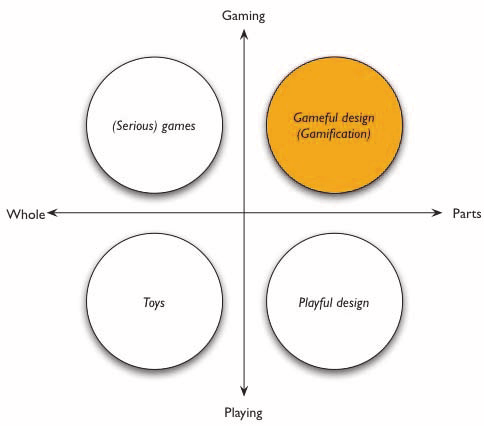
\includegraphics[scale=0.6]{images/gamification_einordnung}
		\caption{Die verschiedenen Arten des Spielens nach \cite{DD2011}.}
		\label{gamification_einordnung}
	\end{center}
\end{figure}

Der Begriff Gamification ist dabei von dem Wort \glqq Gaming \grqq{} abgeleitet.
Gaming bezieht sich dabei auf ein seriöses Spielen.
Dies steht dabei dem \glqq Playing \grqq{} gegenüber (vgl. Abbildung \ref{gamification_einordnung}).
Playing beschreibt nach \cite{Wa2003} ein Spielen in einer offenen Welt, die Oft nur durch die Kreativität der Spieler beschränkt ist.
Der Aufbau der Spielwelt, beispielsweise mit Spielzeugen wie Lego, ist dabei ein zentraler Aspekt.
Gaming unterscheidet sich\cite{DD2011} von Playing dadurch, dass das Gaming einem Regelwerk unterliegt, welches die Teilnehmer beim Erreichen eines gesetzten Ziels einschränkt und somit eine Herausforderung unterliegt.
Am Beispiel Schach verdeutlicht, liegt das Ziel darin, den gegnerischen König zu schlagen, ohne dass der eigene König geschlagen wird.
Einschränkend gilt hierbei, dass die Spieler immer abwechselnd ziehen und die Figuren in ihrer Beweglichkeit eingeschränkt sind.
Zusätzlich gibt es teilweise noch eine zeitliche Einschränkung, sodass für alle Züge zusammen in Summe nur eine gewisse Zeit zur Verfügung steht.

Gamification ist die Übertragung von Elementen aus dem Gaming in Bereiche, die nicht mit dem Spielen oder der Unterhaltung generell verwandt sind.
Am Beispiel Joggen verdeutlicht bedeutet das, dass als Ziel eine vorher festgelegte Distanz pro Woche definiert wird.
Die Möglichkeiten, dieses Ziel zu erreichen, werden dadurch eingeschränkt, dass zum Erreichen nur eine festgelegte Zeit zur Verfügung steht und der Spieler gegebenenfalls die zu erreichende Distanz nicht in einem Mal zurücklegen kann und von daher mehrere Läufe aufsummieren muss.

\subsection{Spielermotivation}
\label{Spielermotivation}
Motivation ist laut \cite{SH2014} ein psychologischer Prozess, der ein zielgerichtetes Handeln initiieren oder verstärken kann.
Für die Effektivität von Gamification ist entscheidend, dass beim Spieler Motivation generiert wird, das gesetzte Ziel zu erreichen.
Dazu kann das Fördern von Motivation aus verschiedenen Perspektiven betrachtet werden, entsprechend gibt es verschiedene Arten auf die Motivation gefördert werden kann.

\paragraph{Bedürfnisse des Spielers}
Spieler haben laut \cite{SH2014} verschiedene Bedürfnisse, die sie erfüllen wollen.
Diese sind dabei abhängig von der Ausprägung unterschiedlicher Charakterzüge eines Spielers.
Generell gibt es das Bedürfnis nach Erfolg, nach Einfluss und Statussymbolen und nach Zusammengehörigkeit.
Dadurch, dass einem Spieler ein Erfolg oder eine Gruppenzugehörigkeit in Aussicht gestellt wird, hat der Spieler nun die Möglichkeit diese Bedürfnisse zu erfüllen und er wird versuchen, die notwendigen Anforderungen zu erfüllen.

\paragraph{Positive und negative Eindrücke}
Aus der Betrachtung der verhaltensorientierten Perspektive geht laut \cite{SH2014} hervor, dass positive und negative Eindrücke oder Erfahrungen zukünftiges Verhalten beeinflussen.
Entsprechend kann durch positives und negatives Feedback oder Belohnungen zukünftiges Verhalten gesteuert werden.

\paragraph{Erfüllung von Erwartungen}
Laut \cite{SH2014} ist Motivation aus der kognitiven Perspektive abhängig von den gestellten Erwartungen.
Diese Erwartungen können allgemeingültig sein und beispielsweise anhand des Alters oder der Fähigkeiten oder individuell durch den Spieler festgelegt werden.
Motivation wird dabei durch die Erfüllung beziehungsweise das Bedürfnis nach Erfüllung dieser Erwartungen generiert.

\paragraph{Selbstverwirklichung}
Selbstverwirklichung ergibt sich nach \cite{SH2014} aus den Bedürfnissen nach Autonomie, Kompetenz und sozialer Verbundenheit.
Die Erfüllung dieser Bedürfnisse fördert laut \cite{SH2014} die intrinsische Motivation des Spielers.

\paragraph{Nutzerinteressen}
Aus der Interessensperspektive berücksichtigt laut \cite{SH2014} individuelle Vorlieben und inhaltliche Aspekte.
Motivation ergibt sich demnach aus der Beziehung des Spielers zu der Aufgabe oder dem Kontext.
Idealerweise kann dies laut \cite{SH2014} zu einem vollständigen Eintauchen in die Aufgabe führen, dem sogenannten \glqq Flow \grqq{}.
\cite{Zi2011} erklärt Flow als einen Zustand, in dem der Anspruch einer Aufgabe den Fähigkeiten des Spielers entspricht.
Übersteigen die Fähigkeiten den Anspruch, langweilt sich der Spieler und er ist weniger motiviert. Übersteigt der Anspruch die Fähigkeiten hingegen, gerät der Spieler unter Leistungsdruck und er sorgt sich um die Erfüllung der Aufgabe, was laut \cite{As2000} bis hin zu Angstzuständen führen kann.
Auch dadurch sinkt die Motivation des Spielers.
Das Erreichen der Flow-Zone, in der die Fähigkeiten den Ansprüchen entsprechen, erfordert demnach ein genaues Abstimmung dieser beiden Aspekte.

\paragraph{Emotionales Empfinden}
Auch über die emotionale Ebene lässt sich laut \cite{SH2014} Motivation generieren.
\cite{As2000} führt an, dass unterschiedlich formulierte Aufgabenstellungen Motivation fördern oder einschränken können.
Demnach lässt sich Motivation durch die Verminderung negativer Emotionen wie Angst, Ärger oder Neid und die Verstärkung positiver Emotionen wie Sympathie oder Freude fördern.

\subsection{Gamification-Elemente}
\label{Elemente}
Wichtig dabei ist, dass der Spieler ein Feedback zu seinem aktuellen Fortschritt bekommt.
Am Beispiel Schach ist dies die Stellung der Figuren und somit die Feldhoheit.
Am Beispiel der Gamification von Joggen könnte dies ein Abbild der Gesamtdistanz und ein entsprechender Positionsmarker mit der aktuell zurückgelegten Distanz sein.
Wie oben beschrieben, werden für diese Darstellung Elemente aus dem Gamedesign verwendet.
Im Folgenden werden einige Elemente beispielhaft vorgestellt und ihr Nutzen erläutert.

\paragraph{Punkte}
Punkte dienen laut \cite{SH2014} zur Darstellung der aktuellen Situation.
Sie können auch zur Veranschaulichung von Belohnungen verwendet werden und geben ein direktes Feedback.
Dieses Feedback kann durch das Erhalten von Punkten positiv beziehungsweise durch das Verlieren von Punkten negativ sein.

\paragraph{Badges}
Badges oder Auszeichnungen sind Statussymbole innerhalb der Gamification.
Sie erfüllen das Bedürfnis des Spielers nach Erfolg und Anerkennung (vgl. \cite{SH2014}).
Darüber hinaus fungieren sie laut \cite{SH2014} als eine Form der Gruppenidentifikation, da sie gemeinsame Erfahrungen kommunizieren.
Für Spieler, die ein bestimmtes Badge noch nicht erreicht haben, können sie außerdem als Ziel fungieren, dessen Belohnung dann das Erhalten dieses Badge ist.

\paragraph{Fortschrittsbalken}
Fortschrittsbalken veranschaulichen einen Fortschritt hinsichtlich eines Ziels.
Sie gelten dabei individuell für einen Spieler und zeigen die Erreichbarkeit des jeweiligen Ziels.

\paragraph{Leistungsdiagramme}
Leistungsdiagramme setzten einen individuellen Score in Relation zu anderen Scores.
Diese anderen Scores können von anderen Spielern oder anderen Zeitpunkten stammen.
Stammen sie von anderen Spielern, zeigt das Diagramm, wie der Spieler sich im Vergleich zu den anderen Spielern im Bezug auf ein Ziel hin entwickelt.
Betrachtet das Diagramm hingegen unterschiedliche Zeitpunkte des selben Spielers, liegt der Fokus auf der Verbesserung der Fähigkeiten des Spielers und fördert das Meistern dieser (vgl. \cite{SH2014}). 

\paragraph{Quests}
Quests sind laut \cite{SH2014} kleine Aufgaben oder Herausforderungen mit einem klar definierten Ziel.
Der Fortschritt auf dieses Ziel hin muss dabei transparent sein, sodass es für den Spieler ersichtlich ist, welche Konsequenzen sein Aktionen im Bezug auf das Erreichen des Ziels haben.
Das Erreichen dieses Ziels ist dabei immer mit einer Belohnung verknüpft.

\paragraph{Avatare und Profile}
Avatare beziehungsweise Profile und die Entwicklung dieser repräsentieren den Spieler.
Spieler können eine Verbundenheit zu ihren Avataren entwickeln, sodass ein Fortschritt des Avatars einen persönlichen Fortschritt bedeutet (vgl. \cite{SH2014}).

\paragraph{Leaderboards}
Leaderboards oder Bestenlisten stellen den Erfolg der Spieler an der Spitze dar.
Spieler, die nicht an der Spitze stehen, könnten allerdings demotiviert werden, da ihre schlechteren Leistungen veröffentlicht werden (vgl. \cite{SH2014}).
Dies führt dazu, dass der Einsatz von Leaderboards kritisch zu sehen ist.
Durch die Verwendung von Team-Leaderboards können diese negativen Effekte allerdings etwas reduziert werden, da sie den Fokus auf die Teamleistung legen.
Zum einen wird dadurch kein einzelner Spieler bloßgestellt und zum anderen hat das Team ein gemeinsames Ziel auf das es hinarbeiten kann, wodurch sich laut \cite{SH2014} die Verbundenheit im Team erhöht. 

\section{Kriterien für qualitativ hochwertigen Code}
\label{Kriterien_guter_Code}
Ein zentraler Aspekt dieser Arbeit ist die Messung von Code-Qualität.
Dazu muss zunächst definiert werden, was im Rahmen dieser Arbeit unter qualitativ hochwertigem Code verstanden wird.
Laut \cite{ISO-25010} sind das folgenden Aspekte.
Einige dieser Aspekte lassen sich nicht ohne Kenntnis über den Projektkontext oder oder die Ausführung des Programms im laufenden Betrieb bewerten.

\subsection{Funktionale Vollständigkeit}
Die funktionale Vollständigkeit beispielsweise ist immer von den Anforderungen innerhalb des Projekts abhängig.
Ohne Kenntnisse über diese Anforderungen lassen sich auch keine Aussagen über den Erfüllungsgrad dieser Anforderungen und somit über die funktionale Vollständigkeit treffen.
Darüber hinaus ist die Überprüfung von Semantik innerhalb der Software nur sehr schwer möglich, da dafür Intelligenz notwendig ist, die ein Computerprogramm nicht liefern kann.
Des weiteren ist es nicht möglich, zu prüfen, ob ein Programm fehlerfrei ist, es lässt sich lediglich validieren, dass ein Programm für eine gegebene Liste an Eingaben die gewünschten Ausgaben erzeugt (vgl. \cite{Di1972}).

\subsection{Nutzbarkeit}
Die Aspekte Nutzbarkeit, Erlernbarkeit und Barrierefreiheit beziehen sich auf die Benutzeroberfläche des Programms.
Da eine in Java\footnote{\url{https://java.com/de/}} geschriebene Benutzeroberfläche nur in einigen Anwendungen vorhanden ist, können hier nur schwer gerechte Bewertungen vorgenommen werden, da viele Projekte nicht in diesem Aspekt bewertet werden können.
Die Bewertung von Projekten, die für die Benutzeroberfläche nicht Java verwenden oder keine Benutzeroberfläche haben, wäre verzerrt, da ein Ausgleich für die in diesem Kriterium vergebenen Punkte geschaffen werden müsste.
Daher wird im Rahmen dieser Arbeit der Aspekt der Nutzbarkeit vernachlässigt.

\subsection{Performanz}
Auch ist es schwer, die Performanz und den Ressourcenverbrauch einer Funktion zu ermitteln, ohne den semantischen Hintergrund zu kennen oder die Funktion auszuführen.
Einige Aspekte des Ressourcenverbrauchs, beispielsweise Netzwerklast oder Speicherverbrauch, lassen sich nur schwer voraussagen und müssen im laufenden Betrieb gemessen werden.
Daher wird dieser Aspekt im Rahmen dieser Arbeit vernachlässigt.

\subsection{Kompatibilität}
Auf die Kompatibilität zu anderer Software können in hier nur schwer Rückschlüsse gezogen werden.
Dafür würden Kenntnisse über diese andere Software benötigt.
Anschließend müssten die Aufrufe und Implementierungen von Schnittstellen untersucht werden.
Java bietet allerdings verschiedene Möglichkeiten, um Schnittstellen zu anderer Software aufzurufen.
Dies kann über \acf{REST}- beziehungsweise \acf{SOAP}-Anfragen, für die es verschiedene Implementierungen gibt, als auch über das Importieren dieser anderen Software als Abhängigkeit geschehen.
Die Entwicklung der Muster zur Erkennung dieser Aufrufe und Implementierungen geht dabei über den zeitlichen Rahmen dieser Arbeit hinaus.
Auch zur Koexistenz neben anderen Systemen lassen sich nur schwer Aussagen tätigen, da das Programm hierzu im laufenden Betrieb untersucht werden muss.

\subsection{Zuverlässigkeit}
Die Zuverlässigkeit von Software lässt sich durch Codeanalysen gut bewerten.
Zum einen kann unter dem Aspekt des Reifegrads des Programms die Testabdeckung untersucht werden.
Durch eine hohe Testabdeckung kann erreicht werden, dass die Methoden das machen, was sie sollen.
Dabei muss aber auch darauf geachtet werden, dass die Tests dazu geeignet sind, den Code zu testen.
Es ist auch möglich, eine hohe Testabdeckung zu erreichen, ohne dass die Funktionsweise tatsächlich geprüft wurde.
Die Testabdeckung besitzt dementsprechend nur eingeschränkte Aussagekraft zur Zuverlässigkeit der Software.

Ein weiterer Aspekt der Zuverlässigkeit ist die Fehlertoleranz.
Damit eine Anwendung Tolerant gegenüber Fehlerfällen ist, müssen diese Fehlerfälle erkannt und durch eine alternative Abarbeitungsvariante behandelt werden können.
Fehlerfälle wie beispielsweise invalide Nutzereingaben können innerhalb der statischen Codeanalyse durch entsprechend gewählte Testfälle überprüft werden.
Dies setzt allerdings voraus, dass solche Tests existieren.
Es müsste also gezeigt werden, dass das Programm fehlerfrei ist, was nach \cite{Di1972} nicht möglich ist.
Auch die Toleranz gegenüber Fehlern außerhalb des Programms, beispielsweise Netzwerkfehler, Stromausfälle oder Speicherfehler, sind ein Aspekt der Fehlertoleranz.
Innerhalb einiger Frameworks gibt es hierfür teilweise Maßnahmen, Spring\footnote{\url{https://spring.io/}} bietet hier beispielsweise den Cirquit Breaker\footnote{\url{https://spring.io/projects/spring-cloud-circuitbreaker}}.
Es könnte in den Fällen, in denen solche Frameworks verwendet wurden, eine Validierung stattfinden, dieser Sonderfall ist aber zu speziell als dass er in dieser Arbeit berücksichtigt werden soll.

Die Wiederherstellbarkeit ist ein weiterer Bereich innerhalb der Zuverlässigkeit.
Sie wird allerdings hauptsächlich vom System auf dem das Programm ausgeführt wird beeinflusst.
Maßnahmen an dieser Stelle sind beispielsweise eine geeignete Backup-Strategie oder die Replikation einzelner der Anwendung oder einzelner Teile dieser.
Entsprechend wird die Wiederherstellbarkeit für die Messung der Codequalität hier auch nicht berücksichtigt.

\subsection{Sicherheit}
Die Sicherheit eines Programms ist in \cite{ISO-25010} definiert als Grad zu dem das Programm Daten vor unbefugten Zugriffen schützt.
Das Programm nun dahingehend zu analysieren, dass alle Funktionen mit den entsprechenden Zugriffsbeschränkungen versehen worden sind, ist wieder eine semantische Überprüfung und somit nur schwer umzusetzen.
Dies gilt auch für die Validierung, ob vor jedem Zugriff eine Authentifizierung korrekt erfolgt ist.

Die Nachverfolgbarkeit von Aktionen innerhalb des Programms ist ein weiterer Aspekt der Sicherheit.
Hierzu gehört zum einen, das belegt werden kann, dass eine Aktion oder ein Ereignis stattgefunden hat und zum anderen wer diese Aktion ausgeführt hat.
Im Programm können hierzu beispielsweise Log-Ausgaben verwendet werden.
Um mit Hilfe von Mustererkennung im Code zu validieren, dass entsprechende Ausgaben getätigt werden, müssten 
diese Muster zur Erkennung von Befehlen zum Ausführen von Log-Ausgaben entwickelt werden, was den zeitlichen Rahmen dieser Arbeit überschreitet.
Im laufenden Betrieb können diese Log-Ausgaben zwar gelesen werden, allerdings ist der laufende Betrieb innerhalb der Codeanalyse nicht möglich.
Darüber hinaus müsste erkennbar sein, wo die Grenzen zwischen den einzelnen Aktionen sind, sodass bewertet werden kann, ob eine Log-Ausgabe für eine Aktion getätigt wird.
Aufgrund des semantischen Aufbaus der einzelnen Aktionskontexte und der Vielzahl an Implementierungsmöglichkeiten zum Ausgeben von Log-Informationen ist die Analyse hier sehr komplex und wird im Rahmen dieser Arbeit nicht berücksichtigt.

Ein Möglichkeit, die Sicherheit eines Programms innerhalb einer Codeanalyse zu bewerten, ist die Analyse auf Schwachstellen.
Hierzu kann eine \acf{OWASP}-Top-Ten-Analyse verwendet werden. 
Die \acs{OWASP}-Top-Ten ist eine Liste mit den zehn kritischsten Sicherheitsbedenken für Web-Applikationen (vgl. \cite{Ow2020}).
Dadurch können potentielle Sicherheitslücken innerhalb des Programms aufgedeckt werden.

\subsection{Wartbarkeit}
Die Wartbarkeit beschreibt laut \cite{ISO-25010} die Effektivität und Effizienz mit der Modifikationen oder Korrekturen umsetzen lassen.
Dazu gehört unter anderem die Auftrennung des Programms in Module und die entsprechende Wiederverwendbarkeit dieser Module.
Da die Auftrennung des Programms in einzelne Module entlang der semantischen Grenzen geschieht, ist dieser Aspekt nur schwer zu analysieren.
Durch das Zählen von Passagen mit doppeltem Code kann allerdings eine Aussage über die Wiederverwendbarkeit von Funktionen und Modulen getroffen werden.

Ein weiterer Bereich ist die Analysierbarkeit und Modifizierbarkeit.
Diese Aspekte beschreiben den Grad zu dem Änderungen einen Einfluss auf die Korrektheit des Programms haben beziehungsweise voraussichtlich haben werden.
Um entsprechende Aussagen tätigen zu können, ist es wichtig, die einzelnen Programmteile mit ihren Funktionen und eventuellen Seiteneffekten zu verstehen.
Hierbei hilft wie oben beschrieben die Einhaltung von Stilrichtlinien und Konventionen, welche innerhalb einer statischen Codeanalyse sehr gut gemessen werden kann.

Ein weiterer Aspekt in der Analysierbarkeit ist das Wissen um den Code.
Je komplexer der Code ist, desto schwerer wird es, ihn zu verstehen.
Die Komplexität lässt sich dabei innerhalb einer statischen Codeanalyse mit beispielsweise der McCabe-Metrik messen (vgl. \cite{MC1976}).

Auch die Verteilung von Wissen um den Code innerhalb des Entwicklungsteams gehört zur Analysierbarkeit.
Je weniger Teammitglieder sich in einem Teil des Codes auskennen, desto geringer ist das Verständnis des Codes.
Wenn es soweit kommt, dass sich nur noch ein Teammitglied in einem Teil des Codes auskennt, besteht ein Wissensmonopol.
Sollte es dazu kommen, dass dieses Teammitglied nun beispielsweise auf Grund von Krankheit oder Urlaub nicht erreichbar ist, müssen sich die anderen Teammitglieder erneut einarbeiten, was sich negativ auf die Analysierbarkeit auswirkt.

\subsection{Portierbarkeit}
Die Portierbarkeit beschreibt, wie gut sich ein Programm von einem System auf ein anderes transferieren lässt.
Die Systeme können sich dabei beispielsweise in der verbauten Hardware, der Laufzeitumgebung oder der Prozessorarchitektur unterscheiden.
Da es sich bei dem Code, den coderadar analysieren kann, um Java-Code handelt, sind die Programme automatisch weitestgehend unabhängig vom Betriebssystem, da es für unterschiedliche Betriebssysteme unterschiedliche Ausführungsumgebungen gibt.
Für Unterschiede wie unterschiedliche Separatoren in Dateipfaden bietet Java ebenfalls Lösungen.
Die verbaute Hardware spielt an der Stelle für das Programm lediglich leistungstechnisch eine Rolle, da die Laufzeitumgebung von Java die Hardwarestruktur entsprechend abstrahiert.

Ein weiter Aspekt in der Portierbarkeit ist die Installierbarkeit.
Sie beschreibt den Grad der Effektivität und Effizienz, mit dem das Programm installiert beziehungsweise deinstalliert werden kann.
Dies ist immer vom Programm selber und seinen Abhängigkeiten abhängig.
Es gibt verschiedene Möglichkeiten, ein Java-Programm auszuliefern.
Zentral ist dabei aber immer ein Java-Archiv, welches per Konsole ausgeführt werden kann.
Entsprechend muss eine Java-Laufzeitumgebung installiert sein, damit das Programm ausgeführt werden kann.
Dieses Archiv kann beispielsweise innerhalb eines Docker\footnote{\url{https://www.docker.com/}} Images verpackt werden, was zusätzlich noch eine Installation von Docker erfordert.
Alternativ kann das Java-Archiv auf einen Web-Applikationsserver deployt werden, was wiederum die Installation eines solchen Applikationsservers erfordert.
Die Installierbarkeit ergibt sich somit nicht nur aus dem Programm selbst, sondern auch aus den jeweiligen Abhängigkeiten und der Auslieferungsform.
Entsprechend ist es nur schwer möglich, Aussagen über die Installierbarkeit zu treffen.

Die Austauschbarkeit des Programms beschreibt den Grad zu dem das Programm ein anderes Programm, welches dem selben Zweck dient, in der selben Umgebung ersetzen kann.
Um hierzu eine Aussage treffen zu können, wird Kenntnis über das zu ersetzende Programm benötigt.
Daher wird dieser Aspekt im Rahmen dieser Arbeit vernachlässigt.

\subsection{Auswahl der Qualitätskriterien}
\label{Auswahl_Kriterien}
Wie oben beschrieben, eignen sich nicht alle Aspekte aus \cite{ISO-25010} zur Bewertung der Codequalität innerhalb der Codeanalyse.
In diesem Abschnitt werden die Aspekte vorgestellt, die im Rahmen dieser Arbeit als Kriterien für qualitativ hochwertige Software verwendet werden sollen.
Die im folgenden aufgelisteten Metriken stammen aus \cite{Ch2021} und \cite{So2021}.

\paragraph{Zuverlässigkeit}
Die Zuverlässigkeit des Programms wird im Rahmen dieser Arbeit unter anderem anhand der Testabdeckung gemessen.
Der oben beschriebene Fall, dass einige Tests die Funktionsweise des zu testenden Codes nicht korrekt prüfen, wird hier nicht berücksichtigt.
Es wird davon ausgegangen, dass die geschriebenen Tests zur Überprüfung der Funktionsweise geeignet sind.
Die gefundenen Bugs und Code-Smells und der entsprechend geschätzte Aufwand zur Behebung dieser fließen ebenfalls in die Bewertung der Zuverlässigkeit mit ein.

Metriken, die für die Messung der Zuverlässigkeit verwendet werden, sind folgenden:
\begin{itemize}
	\item $test\_success\_density$\\
	Die $test\_success\_density$ gibt den Anteil erfolgreicher Tests in einer Software an.
	Je mehr Tests fehlschlagen, desto unzuverlässiger ist Programm 
	\item $uncovered\_lines$\\
	$uncovered\_lines$ gibt an, wie viele Programmzeilen nicht im Rahmen von Tests ausgeführt werden.
	Sollte diese Zeilen einen Fehler beinhalten, kann dieser nicht durch Tests gefunden werden.
	\item $line\_coverage$\\
	Die $line\_coverage$ beschreibt den Anteil an Zeilen, die durch Tests abgedeckt sind.
	\item $coverage$\\
	$coverage$ beschreibt eine Mischung aus Zeilenüberdeckung und Bedingungsüberdeckung und gibt so noch besser Aufschluss darüber, welcher Code durch Tests abgedeckt ist.
	\item $effort\_to\_reach\_maintainability\_rating\_a$ % TODO existiert die Metrik?
	\item $code\_smells$\\
	$code\_smells$ sind potentielle Problemstellen im Code.
	An diesen Stellen ist der Code verwirrend oder schwer zu verstehen und zu warten.
	Sie müssen nicht zwangsweise zu Fehlern führen, sind aber Stellen, auf die der Entwickler besonderes Augenmerk richten sollte, da sie zu unvorhergesehenem verhalten führen können.
	\item $bugs$\\
	$bugs$ sind Fehler im Programmcode, die einer direkten Behebung bedürfen.
	Diese Fehler führen dazu, dass das Programm abstürzt oder falsche Aktionen ausführt.
	\item $reliability\_rating$\\
	Das $reliability\_rating$ bezieht sich auf sich auf die Anzahl und die Schwere der gefundenen Bugs.
	Die Schwere geht dabei von \textit{BLOCKER}, ein Problem welches sofort behoben werden muss, da es zum Absturz des Systems führen kann, bis \textit{MINOR}, was Qualitätsmängel beschreibt, die die Entwicklerproduktivität beeinflussen.
	Zu ersterem gehören unter anderem Speicherlecks, zu letzterem gehören beispielsweise zu lange Zielen, die das Lesen des Codes erschweren.
	\item $violations$\\
	In den $violations$ werden alle Arten von Problemstellen unabhängig von ihrer Schwere zusammengefasst.
	\item $lines\_to\_cover$\\
	$lines\_to\_cover$ beschreibt die Anzahl an Code-Zeilen, die durch Tests abgedeckt werden müssen.
	\item $sqale\_rating$\\
	Das $sqale\_rating$ beschreibt die Zeit die anteilig zur gesamten Entwicklungszeit, die notwendig ist, um technische Schulden im Projekt auszugleichen.
\end{itemize}

\paragraph{Sicherheitsschwachstellen}
Im Rahmen der Analyse der Sicherheit des Programms wird eine Analyse auf mögliche Schwachstellen durchgeführt.
Zu diesen Schwachstellen gehören unter anderem Aspekte aus den \acs{OWASP}-Top-Ten, kommunikationsspezifische Schwachstellen wie offene Cross-Origin-Einstellungen, Sicherheitslücken aus der \acf{CWE} oder sprachspezifische Schwachstellen wie Code-Injektion bei dynamischer Code-Ausführung.

Cross-Origin-Einstellungen sorgen dafür, dass Anfragen an einen Server nur von bestimmten Adressen aus erlaubt sind.
Dadurch kann beispielsweise verhindert werden, dass ein Dienst auf Daten aus dem Speicher des Browsers zugreift und so Anfragen im Namen des Nutzers stellt.

Die \acs{CWE} ist eine Auflistung bekannter Sicherheitslücken in Systemen, Frameworks und Sprachen.
Für viele dieser Sicherheitslücken existieren bereits Lösungen, für andere müssen eigene Lösungen implementiert werden.

Bei der dynamischen Ausführung von Code kann zur Zeit der Kompilierung nicht gewährleistet werden, welche Art von Objekt verwendet wird, dies steht erst zur Ausführungszeit fest.
Ein Angreifer könnte an dieser Stelle nun ein manipuliertes Objekt injizieren und so die Funktion der Software beeinflussen.

Sollten entsprechende Schwachstellen vorhanden sein, senkt dies die Codequalität an dieser Stelle deutlich.

Zur Bewertung werden hier die gefundenen \textit{vulnerabilities} verwendet.
Eine \textit{vulnerability} bezeichnet dabei eine Stelle im Code, die eine Möglichkeit für einen Angriff bietet.

\paragraph{Wiederverwendbarkeit}
Zur Bewertung der Wiederverwendbarkeit von Code innerhalb des Programms wird die Anzahl von doppeltem Code bewertet.
Doppelter Code deutet darauf hin, dass Funktionen innerhalb des Programms hätten zusammengefasst werden können, wodurch potentiell weniger Fehlerquellen bestehen und die Komplexität reduziert werden kann.
Auch die Dokumentation von Methoden, die potentiell wiederverwendet werden können, trägt einen Teil dazu bei, dass besagte Wiederverwendung stattfindet.

Die Wiederverwendbarkeit wird im Rahmen dieser Arbeit mit folgenden Metriken gemessen:

\begin{itemize}
	\item $duplicated\_lines\_density$\\
	Die $duplicated\_lines\_density$ beschreibt den Anteil von sich wiederholenden Code-Zeilen im Vergleich zum gesamten Code.
	Je öfter, gleicher oder ähnlicher Code erneut geschrieben wurde, desto schlechter sind Teile des Programms wiederverwendbar.
	\item $public\_undocumented\_api$ % TODO existiert diese Metrik
	\item $MissingJavadocMethod$
	Damit Code wiederverwendet wird, muss schnell und einfach erkennbar sein, welche Funktion ein bestimmter Teil des Codes erfüllt.
	Dies kann durch eine passende Dokumentation des Codes, der potentiell wiederverwendet werden kann, erleichtert werden.
	$MissingJavadocMethod$ misst, wie oft diese Dokumentation nicht vorhanden ist. 
\end{itemize}

\paragraph{Analysierbarkeit}
Die Analysierbarkeit ergibt sich im Rahmen dieser Arbeit aus dem Grad der Einhaltung von Stilrichtlinien und Konventionen.
Es wird davon ausgegangen, dass nonkonformer Code schwerer zu lesen, zu verstehen und entsprechend zu analysieren ist.
Die Komplexität des Codes und die Dokumentation spielen hier ebenfalls eine Rolle.

Um die Analysierbarkeit bewerten zu können, werden folgende Metriken herangezogen:

\begin{itemize}
	\item $cognitive\_complexity$\\
	Die $cognitive\_complexity$ beschreibt die Komplexität einer Methode.
	Die Berechnung ist an die McCabe-Metrik angelehnt, der Wert ergibt sich aus der Anzahl gewisser Schlüsselwörter innerhalb einer Methode.
	\item $MissingJavadocMethod$
	\item $MethodName, ClassName, usw.$
	Durch diese Metriken wird überprüft, dass Namen für Bezeichner, beispielsweise Methodennamen oder Klassennamen, einem gewissen Schema entsprechen.
	Es kann zwar nicht validiert werden, dass der Name des Bezeichners der Funktion des selbigen entspricht, allerdings erleichtert dieses Schema generell die Lesbarkeit.
\end{itemize}

\paragraph{Komplexität}
Die Komplexität kann mit der McCabe-Metrik gemessen werden.
Die Metrik berechnet für eine Methode einen Komplexitätswert, welcher wie folgt zu interpretieren ist:

\begin{itemize}
	\item <10: niedrige Komplexität
	\item 11 - 20: mittlere Komplexität
	\item 21 - 50: hohe Komplexität
	\item >50: sehr hohe bis undurchschaubare Komplexität
\end{itemize}

Ein hoher Wert hat entsprechend einen negativen Effekt auf die Analysierbarkeit.
Neben der McCabe-Metrik werden auch noch andere Komplexitätsmetriken verwendet.

Um die Komplexität zu messen, gibt es mehrere Möglichkeiten:

\begin{itemize}
	\item $ognitive\_complexity$
	\item $BooleanExpressionComplexity$\\
	Die $BooleanExpressionComplexity$ bezieht sich auf die Komplexität boolescher Ausdrücke.
	Durch Verschachtlungen von Negationen, Und- und Oder-Ausdrücken können diese teils sehr komplex werden.
	Da diese Ausdrücke häufig in \textit{if}- oder \textit{switch}-Abfragen für die Entscheidung verwendet werden, welcher Zweig eines Programms durchlaufen werden soll, ist es wichtig, dass sie gut zu verstehen sind.
	\item $ClassFanOutComplexity$\\
	Die $ClassFanOutComplexity$ beschreibt die Anzahl an Abhängigkeiten einer Klasse oder eines Interface.
	Jede Abhängig kann dazu führen, dass mehr Code ausgeführt wird, der potentiell zum Verständnis der aktuellen Funktion notwendig ist.
	Je mehr Abhängigkeiten eine Klasse oder ein Interface hat, desto höher ist also auch die Komplexität.
	\item $CyclomaticComplexity$\\
	Die $CyclomaticComplexity$ misst die McCabe-Komplexität.
	\item $NPathComplexity$\\
	Die $NPathComplexity$ ist eine Erweiterung der $CyclomaticComplexity$, bei der stärker auf die Kombination boolescher Ausdrücke eingegangen wurde.
	\item $JavaNCSS$\\
	$JavaNCSS$ beschreibt die Anzahl an Anweisungen innerhalb einer Klasse oder Methode.
	Je mehr Anweisungen vorhanden sind, desto höher ist die Komplexität.
\end{itemize}

\paragraph{Wissensmonopole}
Wie oben beschrieben, sorgen Wissensmonopole dafür, dass Codeverständnis gegebenenfalls neu erarbeitet werden muss.
Grade im Zusammenhang mit komplexem Code ist dies ein Problem.
Durch die Verwendung von Kommentaren und weiterer Dokumentation kann Wissensmonopolen ein Stück weit entgegengewirkt werden.
Wissensmonopole in komplexem Code haben dementsprechend einen negativen Einfluss auf die Analysierbarkeit.

\section{Codeanalyse}
\label{Codeanalyse}
In diesem Abschnitt wird genauer auf die Codeanalyse eingegangen.
Dazu wird zunächst in Abschnitt \ref{Analyseprozess} der Analyseprozess innerhalb von coderadar beschrieben.
Anschließend wird in Abschnitt \ref{Herausforderungen} auf besondere Herausforderungen bei der Erweiterung des bisherigen Analyseprozesses eingegangen.

\subsection{Analyseprozess}
\label{Analyseprozess}
Die Codeanalyse in coderadar erfolgt jeweils Commit- und Dateiweise.
Für jeden Commit werden die Dateien geladen, die geändert wurden.
Diese Dateien werden dann in die konfigurierten Analyse-Plugins gegeben.
Die Plugins implementieren dabei jeweils eine Analysemethode, die als Parameter den Pfad zur Datei und den Dateiinhalt bekommt.
Diese Methode gibt die Metriken für die Datei mit den jeweils berechneten Werten und den Fundorten für die Makel im Quellcode, die zu Abwertungen geführt haben.
Um die Bewertungen für einen Commit zu ermitteln, werden für die Metrikwerte für alle geänderten Dateien in diesem Commit zusammengerechnet.
Dadurch, dass diese Analyse für jeden Commit durchgeführt wird, entsteht auch eine Historie über die Commits.


\subsection{Herausforderungen}
\label{Herausforderungen}
Um einige der in Abschnitt \ref{Kriterien_guter_Code} geforderten Metriken messen zu können, muss die bisher durchgeführte Analyse erweitert werden.
Ein zur Messung dieser Metriken geeignetes Werkzeug ist beispielsweise SonarQube\footnote{\url{https://www.sonarqube.org/}}.
SonarQube bietet mit dem SonarScanner\footnote{\url{https://docs.sonarqube.org/latest/analysis/scan/sonarscanner/}} \acf{CLI} ein Werkzeug für die Kommandozeile, um Projekte zu analysieren.
Das Ergebnis dieser Analyse wird anschließend an einen SonarQube-Server geschickt und kann dort entweder über die Benutzeroberfläche oder eine \acs{REST}-Schnittstelle eingesehen werden. 
An dieser Stelle wird SonarQube verwendet, da es zum einen weit verbreitet ist.
Laut \cite{SC2021} wurden allein in der \glqq as a Service\grqq{}-Version SonarCloud\footnote{\url{https://sonarcloud.io/}}, die ausschließlich für Open-Source-Software genutzt werden kann, bereits über 180.000 Projekte analysiert.
Dazu kommen noch von Firmen und Privatpersonen bereitgestellte Instanzen, die für Closed-Source-Software benötigt werden.
Zum anderen wird SonarQube als Standard bei der adesso SE verwendet wird.
An dieser Stelle orientiert sich diese Arbeit am Vorgehen der adesso SE, da im Rahmen der Masterarbeit, die auf dieser Arbeit aufbauen wird, bei der adesso SE ein Feldversuch zur Evaluierung der in dieser Arbeit vorgenommenen Implementierung durchgeführt werden soll.

An dieser Stelle bestehen aber auch einige Probleme.
Zum einen hält SonarQube, abgesehen von einer manuell vorzunehmenden Versionierung, nur die aktuellen Analyseergebnisse vor.
Um Analyseergebnisse von älteren Commits zu erhalten, muss für den jeweiligen Commit entweder eine Version angelegt werden oder das Projekt muss auf diesen Commit gesetzt werden.
Um an dieser Stelle auch parallele Analysen zu ermöglichen, werden jeweils neue Projekte für die einzelnen Commits angelegt, die über den Commit-Hash eindeutig identifiziert werden.

Eine weitere Herausforderung besteht darin, aus der einzelnen Datei, die in coderadar für die Analyse zur Verfügung steht, den kompletten Projektstand zu bekommen.
Hierfür muss das komplette Projekt an dem zu analysierenden Commit ausgecheckt werden.
coderadar bietet hier die Möglichkeit, die Analyse-Plugins zu konfigurieren.
Hier kann zu Beginn jeder Analyse der entsprechende Commit ausgecheckt werden.

Um nun die SonarQube-Analyse durchzuführen, werden allerdings die kompilierten Dateien benötigt.
Um das Projekt kompilieren zu können, sind zunächst einige Informationen über die Projektstruktur notwendig.
Projekte verwenden teilweise Build-Management-Werkzeuge wie Gradle\footnote{\url{https://gradle.org/}} oder Maven\footnote{\url{https://maven.apache.org/}}.
Durch diese Werkzeuge können Abhängigkeiten, die über die \acf{JRE} hinaus gehen, automatisch aufgelöst werden.
Können diese Abhängigkeiten nicht aufgelöst werden, kann auch das Projekt nicht kompiliert werden.
Entsprechend können auch Tests fehlschlagen und die Metriken falsche Werte zurückgeben.
Um herauszufinden, ob und wenn ja, welches Build-Management-Werkzeug verwendet wird, kann nach bestimmten Dateien im Projektverzeichnis gesucht werden
Gradle zeichnet sich an dieser Stelle durch eine Datei \textit{build.gradle} aus, bei Maven existiert eine \textit{pom.xml}.
Ist eine dieser Dateien im Projektverzeichnis vorhanden, können die entsprechenden Befehle zum Kompilieren des jeweiligen Build-Management-Werkzeugs verwendet werden.
Sind keine dieser Dateien vorhanden, wird der klassische Java-Befehl zum Kompilieren von Dateien verwendet.

An dieser Stelle treten ebenfalls einige Herausforderungen auf.
Mit der Zeit werden Versionen von Abhängigkeiten, des Build-Management-Werkzeugs oder von Java geändert.
Damit das Projekt weiterhin zuverlässig kompiliert werden kann, muss auf diese Versionsänderungen reagiert werden können.
Haben sich Abhängigkeiten so stark verändert, dass die im Build-Management-Werkzeug angegebene Version nicht mehr verfügbar ist, kann das Projekt auch nicht mehr kompiliert werden.
An der Stelle können dann keine Metriken über SonarQube bezogen werden.
Generell kann auf neuere Versionen in den Abhängigkeiten nicht reagiert werden, da in den Abhängigkeiten teilweise benötigte Funktionen geändert werden oder wegfallen, sodass die ursprüngliche Funktionalität der Software nicht mehr gegeben ist.
Darüber hinaus würden solche Änderungen Änderungen in der \textit{build.gradle} oder der \textit{pom.xml} erfordern und somit die Software verändern, was im Rahmen dieses Projekts nicht passieren soll.

Der Anpassung der Version des Build-Management-Werkzeugs kann im Beispiel von Gradle damit begegnet werden, dass ein Gradle Wrapper\footnote{\url{https://docs.gradle.org/current/userguide/gradle_wrapper.html}} verwendet wird.
Dieser zieht die Versionsnummer für Gradle fest, lädt diese herunter und konfiguriert sie.
Dadurch muss nicht jede benötigte Gradle-Version manuell heruntergeladen werden.
Teilweise kann es hier auch passieren, dass die Java-Version, die von Gradle verwendet wird, eine andere ist, als die, die im Projekt verwendet wird.
Dies führt dazu, dass beispielsweise die Java-Version 7 ausgelesen wird, Gradle aber die Version 8 benötigt.
Da laut \cite{OB2021} Java 8 Rückwärtskompatibel zu Java 6 und 7 ist, wird an dieser Stelle immer Java 8 verwendet wenn eine dieser drei Versionen ausgelesen wurde.

Eine Änderung in der Java-Version kann in einem Gradle-Projekt darüber erkannt werden, dass sich bestimmte Eigenschaften in der \textit{build.gradle} ändern.
Hier muss entsprechend eine Version der jeweiligen \acs{JRE} installiert sein, damit das Projekt mit der korrekten Version kompiliert werden kann.
Um die Java-Version entsprechend zu setzen, müssen die Umgebungsvariablen \textit{$JAVA\_HOME$} und \textit{$PATH$} angepasst werden.

Im Anschluss an das Kompilieren des Projekts wird die SonarQube-Analyse gestartet.
Das SonarScanner \acs{CLI} stellt die Analyseergebnisse nicht in Form einer Datei zur Verfügung, sondern lädt diese auf einen SonarQube-Server hoch.
Dieser Server muss neben der Datenbank für coderadar und coderadar selbst deployt werden.
Die Analyseergebnisse können dann, wie oben bereits erwähnt, über eine \acs{REST}-Schnittstelle abgefragt werden.
Damit das Anfragen der Analyseergebnisse möglich ist, muss im SonarQube-Server zunächst ein Projekt für diesen Commit angelegt werden.
Dies ist auch über die \acs{REST}-Schnittstelle möglich und muss zu Beginn einer jeden Analyse gemacht werden.
Im Anschluss an die Analyse kann das jeweilig konfigurierte Projekt dann wieder entfernt werden, um Ressourcen zu schonen.

Damit nicht für jede Datei, die im zu untersuchenden Commit geändert wurde, eine Anfrage gestellt werden muss, wird zu Beginn eine große Anfrage an den SonarQube-Server gestellt.
Die Ergebnisse dieser Anfrage werden dann nach dem jeweiligen Dateipfad aufgeschlüsselt gespeichert.
In der Analyse der jeweiligen Datei wird dann auf diese zwischengespeicherten Daten zugegriffen.
So muss nicht für jede zu analysierende Datei eine Anfrage via \acs{REST} gestellt werden, und die Analyse einer Datei ist performanter.


\chapter{Projektkontext}
\label{Projektkontext}
Dieses Kapitel beschäftigt sich mit der Aufarbeitung der Problemstellung.
Dazu wird zunächst in Abschnitt \ref{Problembeschreibung} das Problem genauer ausformuliert.
Anschließend wird in Abschnitt \ref{Kontext} das Problem in den Kontext von coderadar eingeordnet.
Auf dieser Basis werden dann in Abschnitt \ref{Anforderungen} die Anforderungen an die zu entwickelnden Erweiterungen in coderadar gestellt.
Abschließend erfolgt die wissenschaftliche Einordnung der Arbeit in bereits bestehende Werke.

\section{Problembeschreibung}
\label{Problembeschreibung}
Zwei Eigenschaften von Entwicklern sind nach \cite{WCSP1996}, dass sie faul und hochmütig sind.
Zum einen halten sie ihren eigenen Code oft für qualitativ sehr gut und zum anderen wollen sie wegen ihrer Faulheit bereits geschriebenen Code nicht noch einmal bearbeiten müssen.

Dazu kommt, dass Projekte oft unter Zeitdruck oder mit nur sehr geringem Budget entwickelt werden.
Nach einer Studie von \cite{KPME2002} wurden die Zeitaufwände für etwa ein drittel der untersuchten Projekte zu gering eingeschätzt, lediglich knapp die Hälfte der untersuchten Projekte hatten einen geringeren zeitlichen Aufwand als zu Beginn geschätzt.

Dies führt dazu, dass oft wenig Zeit dafür bleibt, auf qualitativ hochwertigen Code zu achten.
Stattdessen wird oft die schnellere, dafür meist aber auch unsauberere Variante bevorzugt.
Dazu gehört, dass keine Dokumentation, beispielsweise über JavaDoc, erstellt wird, dass mehrere fachlich nicht zusammengehörende Funktionalitäten in einer Klasse implementiert werden oder das einheitliche Stylingrichtlinien außer acht gelassen werden. 

Wie bereits in Abschnitt \ref{Motivation} erwähnt, steigt dadurch der Aufwand, der zum Verstehen der Software notwendig ist.
Somit steigen auch die Kosten, für die entsprechende Projektphase.

Mit der Hilfe von Analysewerkzeugen wie beispielsweise coderadar (vgl. \ref{Kontext}) ist es möglich, entsprechende unsaubere Varianten zu finden.
Die Herausforderung an dieser Stelle ist, wie Eingangs beschrieben, Entwickler dazu zu bringen, direkt qualitativ hochwertigen Code zu schreiben.
Dies dauert zwar erfahrungsgemäß etwas länger, spart dann aber den Aufwand, den Code ein weiteres Mal bearbeiten zu müssen, sodass im Endeffekt Zeit gespart wird.

\section{Kontext coderadar}
\label{Kontext}
coderadar ist ein Analysewerkzeug für Java-Code.
Es dient dazu, automatisiert Codeanalysen auf dem Versionskontrollsystem durchzuführen.
Die Ergebnisse dieser Codeanalysen werden in Form von Metriken festgehalten, die dem Entwicklungsteam bereit gestellt werden.
Darüber hinaus ermöglicht coderadar eine Ansicht der Metriken je Commit, sodass frühere Projektversionen betrachtet werden können.

coderadar verwendet intern verschiedene Plugins zur Codeanalyse.
Bisher sind ein Checkstyle\footnote{\url{https://github.com/checkstyle/checkstyletext}}- und ein \acf{LOC}-Plugin implementiert.
Das Checkstyle-Plugin ist über die Angabe einer Checkstyle-Konfigurationsdatei konfigurierbar.
Ein Vorteil von Checkstyle an dieser Stelle ist, dass Checkstyle im Gegensatz zu anderen Analysewerkzeugen wie beispielsweise SonarQube\footnote{\url{https://github.com/SonarSource/sonarqube}} dateibasiert arbeitet.
Dadurch ist es möglich, den Dateiinhalt aus einem Commit zu laden und zu analysieren.

Die Architektur von coderadar erlaubt es, zusätzlich zu den bereits bestehenden Analyse-Plugins, eigene Plugins zu schreiben.
Diese können per Anwahl einer Checkbox in der Benutzeroberfläche zu- oder abgewählt werden.
Damit im Rahmen dieser Arbeit ein Vergleich zwischen den einzelnen Projekten möglich ist, sollen im Rahmen der Fallstudie später die beiden verfügbaren Plugins verwendet werden.

Neben den Möglichkeiten zu Codeanalyse bietet coderadar eine Nutzerverwaltung.
Ein Nutzer kann ein Projekt anlegen und analysieren lassen.
Dazu werden eine GitHub\footnote{\url{https://github.com}}-URL, ein Projektname und, falls gewünscht, ein Start- und ein Enddatum für die Analyse angegeben.
Im nächsten Schritt können dann die zu verwendenden Analyse-Plugins ausgewählt werden.
Dafür wird ein Muster für zu analysierende Dateien angegeben.
coderadar untersucht dann alle Commits im genannten Zeitraum auf Dateien, die dem angegebenen Muster entsprechen.
Wird eine entsprechende Datei gefunden, wird sie mit den konfigurierten Analyse-Plugins untersucht, und entstehenden Metriken werden zu dem Commit hinzugefügt.
Ein Nutzer kann ein erstelltes Projekt auch für andere Nutzer zur Kollaboration freigeben.

% TODO Screenshots in den Anhang
Nachdem coderadar ein Projekt geclont und analysiert hat, gibt es verschiedene Visualisierungen für die Ergebnisse.
Zum einen können die Rohdaten der Metriken je Commit angezeigt werden.

Darüber hinaus können die Ergebnisse in einer \glqq City-View\grqq{} angezeigt zu lassen (vgl. Abbildung \ref{city_view}).
Dabei wird für jede Änderung in einem Commit ein \glqq Haus\grqq{} erstellt.
Das Aussehen eines solchen Hauses hängt dabei von den vier Faktoren Länge, Breite, Höhe und Farbgebung ab.
Jeder dieser Faktoren lässt sich dabei mit dem Wert einer Metrik belegen.
Die City-View kann sowohl einen Commit als auch zwei Commits vergleichend anzeigen.
Bei der vergleichenden Ansicht besteht die Möglichkeit, entweder beide City-Views nebeneinander oder beide Views in einander anzuzeigen.

Neben der City-View gibt es auch noch eine \glqq Dependency-Map\grqq{} (vgl. Abbildung \ref{dependency_map}).
Die Dependency-Map zeigt die Ordnerstruktur des Projektes sowie die Abhängigkeiten der einzelnen Module untereinander an.
Die einzelnen Unterordner lassen sich dabei noch aufklappen, sodass auch innerhalb eines Unterordners die Abhängigkeiten visualisiert werden.
Auch hier ist sowohl eine Einzelansicht eines Commits als auch eine vergleichende zweier Commits möglich.
Änderungen zwischen den zwei Commits werden entsprechend farblich markiert.

coderadar listet die einzelnen Commits entweder in einer Liste oder in der Baumansicht (vgl. Abbildung \ref{tree_view}) auf.
Die Liste ist nach Erstellungsdatum des Commits sortiert. 
In der Baumansicht werden die Commits anhand der Branches angezeigt, denen sie zugeordnet sind.
Zusätzlich bietet coderadar die Funktion, für einen ausgewählten Commit die Ordnerstruktur und den Dateiinhalt anzuzeigen.

Ein Nutzer kann auch ein Team anlegen.
Innerhalb eines Teams gibt es Mitglieder und Administratoren.
Ein Administrator kann im Namen des Teams ein Projekt anlegen und analysieren.
So ist das Projekt nicht direkt von dem Nutzer abhängig.
Löscht der Nutzer also seinen Account oder verlässt das Team, kann das Team mit dem Projekt immer noch weiterarbeiten.
Ein Nutzer kann dabei auch mehreren Teams angehören.

% TODO diesen Absatz schreiben bei, warum kein Plugin für weitere Analysewerkzeuge entwickelt.
SonarQube hingegen wird als Konsolenwerkzeug oder Plugin für Buildwerkzeuge wie Gradle\footnote{\url{https://gradle.org/}} oder Maven\footnote{\url{https://maven.apache.org/}} ausgeliefert und kann jeweils nur das ganze Projekt zu einem festen Zeitpunkt untersuchen.
Somit ist es deutlich schwerer, Änderungen über Commits nachzuvollziehen.

\section{Anforderungen}
\label{Anforderungen}
In diesem Abschnitt werden die Anforderungen an die im Rahmen dieser Arbeit durchzuführenden Ergänzungen erarbeitet.
An dieser Stelle werden dabei lediglich die funktionalen Anforderungen berücksichtigt, da zum einen die nichtfunktionalen Anforderungen zu einem Teil durch die bestehende Basissoftware abgedeckt sind und zum anderen die nichtfunktionalen Anforderungen für die weitere Arbeit nicht von Bedeutung sind.
Die Identifikation der einzelnen Anforderungen erfolgt über einen Buchstaben und eine Nummer.
Der erste Buchstabe beschreibt dabei, welcher Teil der Anwendung diese Anforderung erfüllen soll.
\glqq A\grqq{} steht dabei für den Analyseprozess, \glqq B\grqq{} für Backend, \glqq F\grqq{} für Frontend.
Die Nummer dient zur Identifikation einer Anforderung im jeweiligen Teilbereich und wird hochgezählt.
Die Anforderungen an den Analyseprozess und die anderen Funktionen des Backends werden hier getrennt betrachtet, da die Ergänzung des Analyseprozesses um die in Abschnitt \ref{Auswahl_Kriterien} gestellten Kriterien Abwägungen zwischen verschiedenen Lösungsansätzen enthalten und somit mit einigem Aufwand verbunden sein werden.

\paragraph{A.1}
Der Analyseprozess für die einzelnen Commits muss dahingehend ergänzt werden, dass der ganze Projektstand an diesem Commit analysiert werden kann und nicht nur die geänderten Dateien.

\paragraph{A.2}
Das System muss eine Möglichkeit zur Untersuchung des Reifegrades des Projekts zum Zeitpunkt des zu analysierenden Commits bieten.
Dazu wird die Testabdeckung innerhalb des Projekts bewertet. Dabei sollen sowohl die Anweisungs- als auch die Zweigüberdeckung berücksichtigt werden.

\paragraph{A.3}
Das System muss eine Möglichkeit zur Untersuchung der Sicherheit des Projekts zum Zeitpunkt des zu analysierenden Commits bieten.
Dazu wird eine \acs{OWASP}-Top-Ten-Analyse verwendet.

\paragraph{A.4}
Das System muss eine Möglichkeit zur Untersuchung der Wiederverwendbarkeit von Teilen des Projekts zum Zeitpunkt des zu analysierenden Commits bieten.
Hierzu wird das Projekt auf doppelten Code hin untersucht.

\paragraph{A.5}
Das System muss eine Möglichkeit zur Untersuchung der Analysierbarkeit des Projekts zum Zeitpunkt des zu analysierenden Commits bieten.
Hierzu soll die Einhaltung von Stilrichtlinien und Konventionen betrachtet werden.

\paragraph{A.6}
Das System muss eine Möglichkeit zur Untersuchung der Komplexität von Teilen des Projekts zum Zeitpunkt des zu analysierenden Commits bieten.
Die Bewertung findet dabei anhand der Komplexitätsmetrik nach \cite{MC1976} statt.

\paragraph{A.7}
Das System muss eine Möglichkeit zur Untersuchung auf Wissensmonopole in Teilen des Projekts zum Zeitpunkt des zu analysierenden Commits bieten.
Dazu wird die Anzahl an Autoren einer Datei zusammen mit der Komplexität nach \cite{MC1976} verwendet.

\paragraph{B.1}
Das System muss für jeden Nutzer eine Gesamtpunktzahl, ein Level, die Punktzahl im aktuellen Level, eine Anzahl an Coins, die Liste absolvierter Quests und die dem Nutzer zugeordneten Contributors speichern.
Ein Contributor ist dabei ein identifizierter Git-Account in einem Projekt.
Einem Nutzer können mehrere Contributors zugeordnet sein, da ein Nutzer zum einen in mehreren Projekten aktiv sein kann und zum anderen mit mehreren Git-Accounts in einem Projekt arbeiten kann.

\paragraph{B.2}
Das System muss für jeden Commit aus den Werten der einzelnen Metriken sowie der Metrikmatrix einen Score berechnen können.

\paragraph{B.3}
Das System muss für jeden Contributor eine Gesamtpunktzahl berechnen.
Diese Gesamtpunktzahl ergibt sich aus der Summe der Scores über alle Commits des Contributors.

\paragraph{B.4}
Das System muss mehrere Level verwalten.
Ein Level hat dabei einen nummerischen Bezeichner, eine Gesamtpunktzahl, die notwendig ist, um dieses Level zu erreichen und die Anzahl an Punkten, die in diesem Level notwendig ist, um das nächste Level zu erreichen.
Mit steigendem Level soll dabei die Anzahl an benötigten Punkten bis zum nächsten Level größer werden.

\paragraph{B.5}
Das System muss Aufgaben, sogenannte Quests, verwalten.
Eine Aufgabe hat einen eindeutigen Identifikator, einen Titel, einen Beschreibungstext, eine Anzahl an Punkten und eine Anzahl an Coins, die ein Nutzer für das Erfüllen bekommt.

\paragraph{B.6}
Das System muss nach der Analyse eines Commits den errechneten Score automatisch zum jeweiligen Nutzer und Contributor dazurechnen.
Bei dem Contributor wird lediglich die Gesamtpunktzahl erhöht.
Bei dem Nutzer muss zunächst die Gesamtpunktzahl erhöht werden.
Reicht die Gesamtpunktzahl aus, um das nächste Level zu erreichen, muss das Level entsprechend hochgezählt werden.
Zusätzlich muss die Punktzahl im aktuellen Level angepasst werden.
Wird ein neues Level erreicht, ist die Punktzahl im aktuellen Level die Anzahl erhaltener Punkte, abzüglich der Punkte, die für den Level-aufstieg nötig waren.
Wird kein neues Level erreicht, werden die erreichten Punkte auf die Punkte im aktuellen Level addiert.

\paragraph{F.1}
Das System muss dem Nutzer sein aktuelles Level, seine Punktzahl im aktuellen Level und die Punktzahl, die im aktuellen Level benötigt wird, in der generellen Übersicht anzeigen.

\paragraph{F.2}
Das System soll eine Übersicht über verschiedene Bestenlisten anzeigen.

\paragraph{F.3}
Das System muss für jedes Projekt eine Bestenliste in der Übersicht der Bestenlisten anzeigen.
Diese Bestenliste wird über die Gesamtpunktzahl der einzelnen Contributors erstellt.
Ist ein Contributor einem Nutzer zugeordnet, muss auch der Nutzername angezeigt werden.

\paragraph{F.4}
Das System muss eine Bestenliste über alle Projekte in der Übersicht der Bestenlisten anzeigen.
Dazu wird für jedes Projekt ein Score errechnet.
Dieser ergibt sich aus der Summe aller Gesamtpunktzahlen aller Contributors des Projekts, geteilt durch die Anzahl an Contributors.
In dieser Bestenliste muss jeweils der Projektname und die Punktzahl angezeigt werden.

\paragraph{F.5}
Das System muss eine Bestenliste über alle Nutzer in der Übersicht der Bestenlisten anzeigen.
Dazu wird jeweils die Gesamtpunktzahl des Nutzers, geteilt durch seine Anzahl an Projekten verwendet.
In der Bestenliste muss je Nutzer der Name, das Level und die Anzahl an Projekten dargestellt werden.

\paragraph{F.6}
Das System muss in einer gesonderten Ansicht die Quests anzeigen.
Dabei sollen in einem Abschnitt die noch nicht abgeschlossenen und in einem anderen Abschnitt die bereits abgeschlossenen Quests des Nutzers aufgelistet werden.

\section{Wissenschaftliche Einordnung}
\label{Wissenschaftliche_Einordnung}
Die Idee, Gamification-Elemente im Zusammenhang mit Code-Qualität zu nutzen, ist nicht neu.
Ein Ansatz ist SonarQuest\footnote{\url{https://www.viadee.de/loesungen/java/sonarquest}}.
SonarQuest nutzt Analyseergebnisse von SonarQube\footnote{\url{https://www.sonarqube.org/}}, um auf Basis eines vordefinierten Regelwerks eine Menge an Kennzahlen und Wartungsaufgaben zu erstellen.
Jeder Nutzer wird durch einen Avatar repräsentiert.
Wie in herkömmlichen Rollenspielen kann ein Nutzer seinen Avatar mit Artefakten ausstatten und der Avatar kann eigene Fähigkeiten ausbilden.
SonarQuest wird dabei immer von einem Gamemaster begleitet, der zu den definierten Wartungsaufgaben jeweils eine Geschichte erstellt.
Daraus resultiert dann jeweils eine Quests, die von einem Spieler angenommen werden kann.
Für das Erfüllen einer Quest und damit einer Wartungsaufgabe bekommt ein Nutzer Gold und Erfahrungspunkte als Belohnung. 
Neben der normalen Belohnung für eine Quest kann der Gamemaster auch Sonderaufgaben und Boni verteilen, um Aspekte wie Teamwork oder Termineinhaltung besonders zu belohnen.\cite{SonarQuest}

SonarQuest ist dabei sehr stark einem klassischen Rollenspiel nachempfunden und bringt somit einigen Mehraufwand mit sich.
Zum einen müssen regelmäßig neue Quests geschrieben werden.
Dabei sollten Quests so geschrieben sein, dass ihre Geschichte den Spieler dazu motiviert, die Aufgabe zu erfüllen.
Laut \cite{SonarQuest} liegt diese Aufgabe jeweils beim Teamleiter.
Dies kann den Teamleiter aber abhängig von der Anzahl an Wartungsaufgaben, Tiefe und inhaltlicher Schlüssigkeit der Geschichten und dem literarischen Talent den Teamleiter sowohl zeitlich als auch in seinen Fähigkeiten überfordern.
Zum anderen basiert die Gamification von SonarQuest ausschließlich auf den Ergebnissen der Analyse von SonarQube.
SonarQube bietet zwar eine Gesamtheitliche Analyse des Projekts, wodurch beispielsweise doppelter Code auch Klassenübergreifend auffällt, allerdings wird für die Analyse mit SonarQube immer das gesamte Projekt benötigt.
Es ist dadurch deutlich komplexer, Unterschiede zwischen zwei Commits herauszustellen oder das Projekt an einem früheren Zeitpunkt in der Entwicklungshistorie zu untersuchen.
Aus diesen Gründen wird in dieser Arbeit SonarQube nicht als Hauptquelle für die Analysedaten verwendet.
Darüber hinaus soll der Aufwand für das regelmäßige Schreiben der Quests wegfallen.
Stattdessen sollen im Vorfeld einige Quests definiert werden, die die Entwickler dann erfüllen können.
Eine Geschichte zu den einzelnen Quests soll es nicht geben.

Ein weiterer Ansatz wird in \cite{Prause2012} vorgestellt. 
Prause et al. haben dazu zwei Gruppen von Studenten untersucht, die jeweils ein ähnliches Softwareprojekt nach agilem Vorgehen in Pair Programming entwickeln sollten.
Beide Gruppen wurden dabei jeweils von Lehrern begleitet.
Der Versuch war dabei in zwei Phasen unterteilt.
In der ersten Phase wurden lediglich Qualitätsmetriken gesammelt und ausgewertet, die Teilnehmer wurden darüber jedoch erst ab der zweiten Phase informiert.
In dieser zweiten Phase wurden die Teilnehmer in einer täglichen Mail sowie in Meetings über den aktuellen Zwischenstand und ihren Punktestand informiert.
Zusätzlich dazu wurden Informationen verschickt, die bei der Verbesserung der Code-Qualität helfen sollten.
Nach Abschluss des Versuchs sollte zudem der Entwickler mit der besten Platzierung einen Amazon-Gutschein erhalten.
Die Bewertung einer Datei fand dabei auf einer Skala von +10 bis -10 statt.

Als Basis für die Bewertung wurde allerdings lediglich die Vollständigkeit des JavaDoc herangezogen.
Dies ist allerdings nur ein Aspekt für qualitativ guten Code nach \cite{ISO-25010}, auf Aspekte wie funktionale Vollständigkeit, Sicherheit oder Performanz wird an dieser Stelle nicht eingegangen.
Die Punktzahl eines Nutzers ergab sich dann daraus, ob er mehr zu positiv oder negativ bewerteten Dateien beigetragen hat.
Zudem weist \cite{Prause2012} selbst die Kritik auf, dass die Bewertungsformel für die Punkte der Teilnehmer undurchsichtig war und somit die Teilnehmer nicht beziehungsweise nur schwer nachvollziehen konnten, wie sie ihre Bewertung verbessern konnten.
Das Pair Programming wird als weiterer Kritikpunkt aufgeführt, da zum einen nur ein Teilnehmer die Anerkennung für die Arbeit beider Partner bekommt und zum anderen für den eigenen Account Beiträge von anderen Entwicklern eingereicht werden können.
Im Rahmen dieser Arbeit sollen mehrere Aspekte aus \cite{ISO-25010} verwendet werden. Außerdem soll die Bewertungsformel einsehbar sein, sodass das Ergebnis nachvollziehbar ist. 

Ein weiterer Versuch wurde von \cite{PJ2015} unternommen.
Ziel dieses Versuchs war es, Gamification einzusetzen, um Stylingrichtlinien durchzusetzen.
Im Rahmen dieses Versuchs sollten zwei Entwicklerteams jeweils ähnliche Software implementieren. 
Als Basis für die Bewertung der Entwickler diente in diesem Versuch eine Punktzahl, die sich aus den mit Checkstyle gemessenen Verstößen gegen die vorgeschriebenen Stylingrichtlinien ergaben.
Die Entwickler wurden dabei sowohl einzeln als auch als Team bewertet.
Der Versuch war in zwei Phasen aufgeteilt, in der ersten Phase bekam Team A Rückmeldung über die Leistung sowohl des Teams als auch der einzelnen Personen, in der zweiten Phase bekam Team B dieses Feedback.
Ein Ergebnis des Versuchs ist, dass beide Teams in der Zeit, in der sie Feedback bekamen, einen deutlich weniger Verstöße gegen die Stylingrichtlinien zu verzeichnen hatten.
Auffällig ist auch, dass die Anzahl an Verstößen bei Team A nach Ende der Feedback-Phase wieder zugenommen hat.
Auch war für die Bewertung des einzelnen Entwicklers sowie des jeweiligen Entwicklerteams die Anzahl an Verstößen lediglich zu Projektende von Bedeutung.
Dies führte dazu, dass Team A kurz vor Ende seiner Feedback-Phase viel Arbeit in die Reduktion der Anzahl an Verstößen gesteckt hat.

Im Rahmen dieser Arbeit soll die Code-Qualität über den gesamten Zeitraum beobachtet werden.
Der Fokus soll nicht auf einer möglichst hohen Code-Qualität sondern auf dem Lernerfolg der Entwickler liegen.
Daher wird die Code-Qualität kontinuierlich betrachtet und wenn möglich sollen individuelle Hilfestellungen zur Verbesserung der Code-Qualität gegeben werden.

\chapter{Entwurf des Lösungsansatzes}
\label{Entwurf}
In diesem Kapitel wird ein Lösungsansatz zur nachhaltigen Steigerung der Codequalität entworfen.
Dazu wird zunächst in Abschnitt \ref{Architektur} die Architektur von coderadar mit der Integration des Lösungsansatzes beschrieben.
In Abschnitt \ref{Metrikmatrix} wird dann auf Basis der Metriken aus \ref{Auswahl_Kriterien} ein Matrix zur Gewichtung der gesammelten Metriken erstellt.
Anschließend wird in Abschnitt \ref{Gamification_Elemente} der Einsatz von Gamification-Elementen ausgearbeitet.

\section{Architektur}
\label{Architektur}

% TODO Codeanalyse nach hier verschieben? Mit Marius besprechen.
Um die weiteren geforderten Metriken erfassen zu können, werden weitere Maßnahmen zu Codeanalyse benötigt.
Dies geschieht in coderadar durch die Ergänzung eines weiteren Analyse-Plugins.
Dazu wird ein neues Untermodul im Modul \textit{coderadar-plugins} angelegt.
Zentraler Aspekt dieses Moduls ist die Klasse \textit{SonarScannerSourceCodeFileAnalyzerPlugin}, welches das Interface \textit{SourceCodeFileAnalyzerPlugin} implementiert.
In coderadar wird via Java Reflection über alle Klassen iteriert, die das \textit{SourceCodeFileAnalyzerPlugin}-Interface implementieren.
Für jede Klasse wird dann die \textit{analyze()}-Methode aufgerufen.
Um die Metriken von SonarQube zu bekommen, wird hier entsprechend ein neues Modul geschrieben, welches eine entsprechende Analyse durchführt.

Darüber hinaus muss jede Analyse vor- und nachbereitet werden.
Zur Vorbereitung gehört das Anlegen des SonarQube-Projekts, das Checkout des zu analysierenden Commits sowie die Analyse ansich.
Zur Nachbereitung gehört das Entfernen des SonarQube-Projekts sowie die Punkteberechnung auf Basis der Metrikwerte und der noch zu erarbeitenden Metrikmatrix.
Die Berechneten Punkte müssen dann dem Autor des Commits gutgeschrieben und sein Level muss angepasst werden.

Die Vor- und Nachbereitung ist jeweils ein Prozess, der von der Dateianalyse getrennt zu betrachten ist, da er nicht je Datei, sondern je Commit durchgeführt werden soll.
Aus diesem Grund wird die Vorbereitung innerhalb der Konfiguration des \textit{SonarScannerSourceCodeFileAnalyzerPlugin} durchgeführt.
Um aus Sicht des \textit{coderadar-core}-Moduls eine Unabhängigkeit zu den einzelnen Plugins herzustellen, wird an dieser Stelle in der \textit{coderadar-plugin-api} ein neues Interface \textit{WrappedAnalyzingProcess} eingeführt.
Dieses Interface schreibt jeweils eine Methode zur Vor- und Nachbereitung der Analyse vor, \textit{prepareAnalysis()} und \textit{postprocessAnalysis()}.
Im Analyseprozess wird dann zunächst über alle Implementierungen des \textit{WrappedAnalyzingProcess} iteriert und für jede Instanz wird die Methode \textit{prepareAnalysis()} aufgerufen.
Anschließend findet die Analyse des Commits, gefolgt von dem Aufruf der Methode \textit{postprocessAnalysis()} für alle Implementierungen des \textit{WrappedAnalyzingProcess}-Interface.

Des weiteren müssen gemäß den Anforderungen aus \ref{Anforderungen} Anpassungen in der Benutzerschnittstelle im Modul \textit{coderadar-ui} vorgenommen werden.
Um die benötigten Daten zu speichern und bereitzustellen, müssen entsprechende Anpassungen in der \acs{REST}-Schnittstelle und dem Datenbankadapter, \textit{coderadar-rest} beziehungsweise \textit{coderadar-graph}, vorgenommen werden.
Für die im Rahmen dieser Arbeit implementierten Erweiterungen müssen darüber hinaus Tests geschrieben werden.
Diese teilen sich auf in Unit-Tests, die im jeweiligen Modul, und Integrationstests, welche im Modul \textit{coderadar-test} implementiert werden.

Entsprechend der in diesem Absatz beschriebenen Änderungen wird coderadar wie im Komponentendiagramm in Abbildung \ref{component_diagram} beschrieben aufgebaut sein.
Orange eingefärbte Module werden dabei geändert, grün gefärbte Module werden hinzugefügt.

\begin{figure}[H]
	\begin{center}
		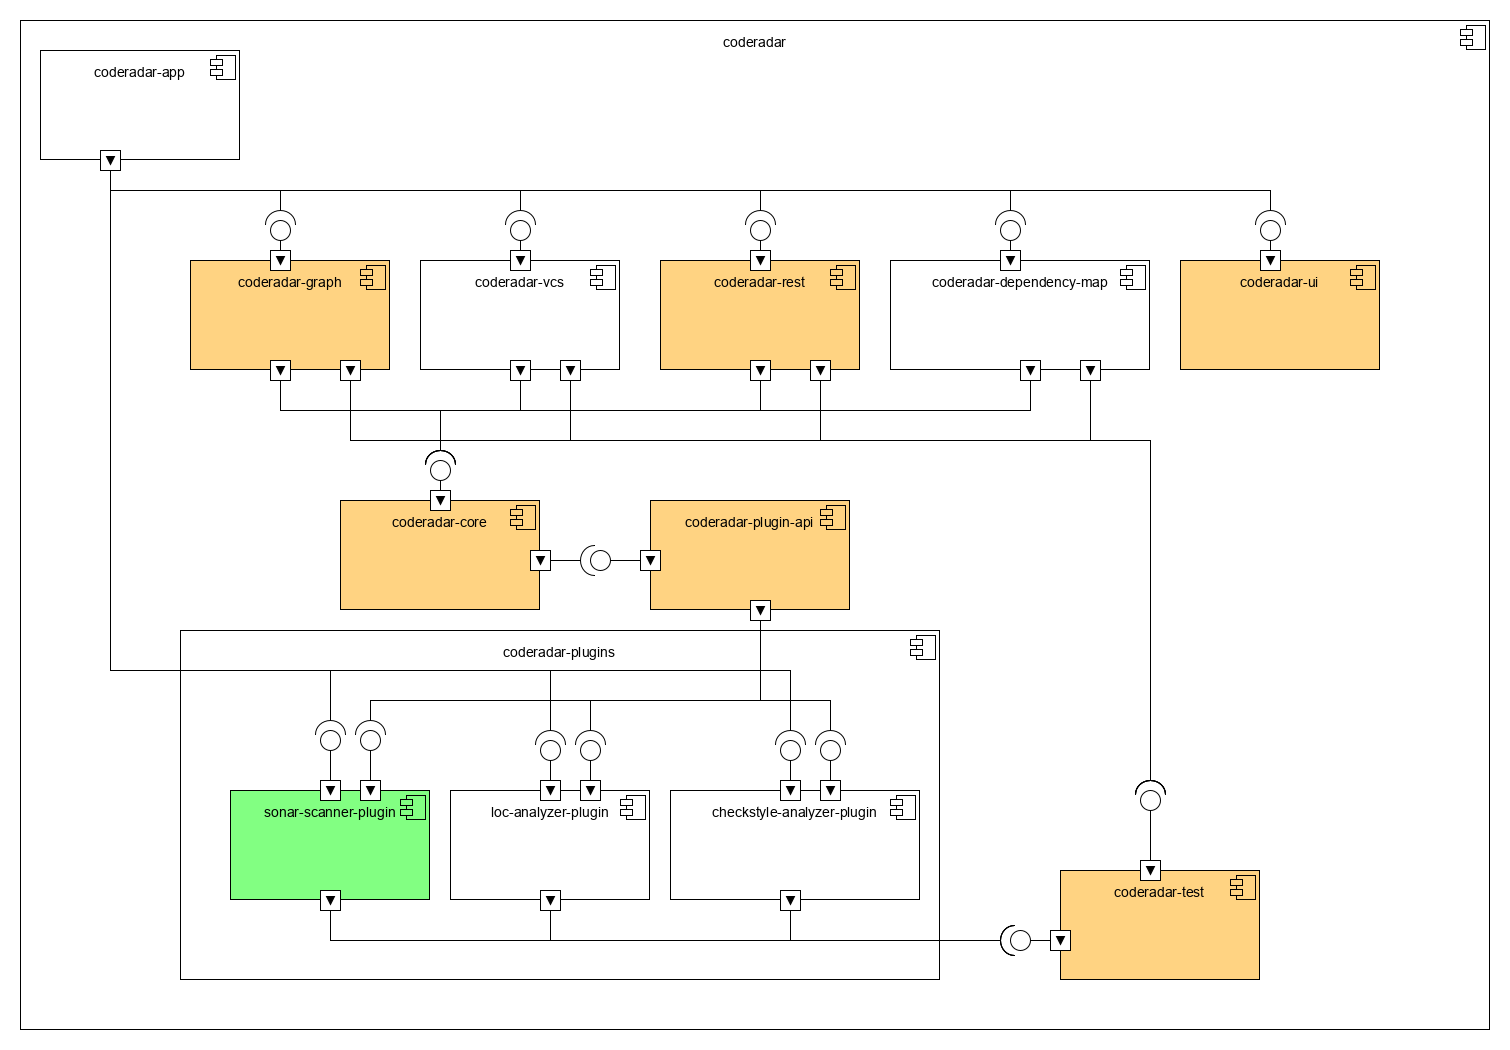
\includegraphics[width=\linewidth]{images/coderadar_components}
		\caption{Die Struktur der Komponenten in coderadar nach den Erweiterungen aus dieser Arbeit.}
		\label{component_diagram}
	\end{center}
\end{figure}

\section{Metrikmatrix}
\label{Metrikmatrix}
Um aus der Menge an Metriken, die coderadar mit der in dieser Arbeit entwickelten Erweiterung für jeden Commit sammelt, eine Summe an Punkten zu ermitteln, müssen die Ergebnisse der Metriken zusammengefasst werden.
Da beispielsweise Vulnerabilities einen deutlich stärkeren Einfluss auf die Qualität des Codes haben, müssen die einzelnen Ergebnisse der Metriken gewichtet werden.
Zur gewichteten Zusammenfassung der Metriken wird an dieser Stelle eine Metrikmatrix verwendet.
Sie multipliziert die Gewichtung der jeweiligen Metrik mit ihrem Wert und erhält in Summe eine Punktzahl für einen Commit.

Eine weitere Aufgabe der Metrikmatrix ist die Ausbalancierung der Punkte, die ein Autor für einen Commit erhalten kann.
Es darf nicht möglich sein, durch das wiederholte Ausführen bestimmter, trivialer Aktionen übermäßig viele Punkte zu erhalten, da sonst die Vergleichbarkeit zu anderen Autoren und Projektteams nicht mehr gegeben ist.
Diese Balancierung wird ebenfalls über die Gewichtung vorgenommen.

Im Folgenden ist diese Metrikmatrix in Tabellenform dargestellt:

\begin{table}[!htb]
	\label{metric_matrix}
	\begin{minipage}{.33\linewidth}
		\centering
		\begin{tabular}{|c|c|}
			\hline
			Metrik & Gewichtung  \\ \hline
			Test & Test \\ \hline
			Test & Test \\ \hline
		\end{tabular}
	\end{minipage}%
	\begin{minipage}{.33\linewidth}
		\centering
		\begin{tabular}{|c|c|}
			\hline
			Metrik & Gewichtung  \\ \hline
			Test & Test \\ \hline
			Test & Test \\ \hline
		\end{tabular}
	\end{minipage}%
	\begin{minipage}{.33\linewidth}
		\centering
		\begin{tabular}{|c|c|}
			\hline
			Metrik & Gewichtung  \\ \hline
			Test & Test \\ \hline
			Test & Test \\ \hline
		\end{tabular}
	\end{minipage} 
	\caption{Metrikmatrix mit der Gewichtung der einzelnen Metriken}
\end{table}

Anhand der in Tabelle \ref{metric_matrix} dargestellten Gewichtsverteilung über die Metriken wird nach der Analyse die Anzahl an Punkten berechnet, die der Autor des Commits bekommt.
Anhand der erhaltenen Punkte wird dann das aktuelle Level des Autors bei Bedarf angepasst.

\section{Gamification-Elemente}
\label{Gamification_Elemente}
Um den Punkte- und Levelstand der einzelnen Autoren aber auch der jeweiligen Projektteams darzustellen, werden verschiedene Gamification-Elemente benötigt.
Im folgenden werden auf Basis der bisherigen Benutzerschnittstelle Prototypen für die Erweiterungen erstellt.
Bei der Konzeptionierung der Prototypen wird besonders auf die beabsichtigte Wirkung der jeweiligen Elemente eingegangen.

\subsection{Punkte}
\label{coderadar_Punkte}
Ein Autor erhält wie bereits erwähnt für das Einreichen eines Commits Punkte.
Dadurch ist es möglich, positive Handlungen beziehungsweise qualitativ hochwertigen Code direkt mit vielen Punkten zu belohnen und qualitativ schlechten Code mit wenig oder keinen Punkten zu bestrafen.
Die Anzahl an Punkten ermöglicht überdies einen einfachen Vergleich zwischen verschiedenen Autoren oder zwischen verschiedenen Zeitpunkten der Betrachtung des Profils eines Autors.
Die Punkte dienen somit auch als Basis für einige der anderen Gamification-Elemente, auf die im Laufe dieses Abschnitts eingegangen wird.
Der Nutzer bekommt seinen aktuellen Punktestand in Form eines Fortschrittsbalken zum nächsten Level angezeigt.

\subsection{Level}
\label{coderadar_Level}
Level dienen als zusätzliche Motivation für den Nutzer, möglichst viele Punkte zu erhalten.
So können mit höherem Level bestimmte optische Zusatzfunktionen freigeschaltet werden.
Der Fortschritt im aktuellen Level wird in den Ansichten, in denen der verfügbare Platz dies zulässt, beispielsweise nicht in der City-View oder der Dependency-Map, an prominenter Stelle mittels eines Fortschrittsbalkens dargestellt.
An dieser Stelle sind folgende Funktionen mit dem entsprechend benötigten Level geplant.

\begin{center}
	\begin{tabular}{|p{12cm}|p{1cm}|}
		\hline
		Zusatzfunktion & Level \\ \hline
		Das persönliche Profilbild kann angepasst werden & x \\ \hline
		Der Fortschrittsbalken für das Level kann alternativ auch den Fortschritt auf ein anderes Ziel hin darstellen & x \\ \hline
		Das Farbschema der Benutzeroberfläche kann angepasst werden & x \\ \hline
		Die Auswahl an Badges, die anderen Nutzern angezeigt werden, kann personalisiert werden & x \\ \hline
	\end{tabular}
\end{center}

\chapter{Umsetzung}
\label{Umsetzung}


\section{Programmierung}
\label{Programmierung}


\chapter{Abschluss}
\label{Abschluss}


\section{Verifizierung der Anforderungen}
\label{Verifizierung_Anforderungen}


\section{Fazit}
\label{Fazit}


\addchap{Anhang} 
\refstepcounter{chapter} 
\begin{figure}[htb]
	\begin{center}
		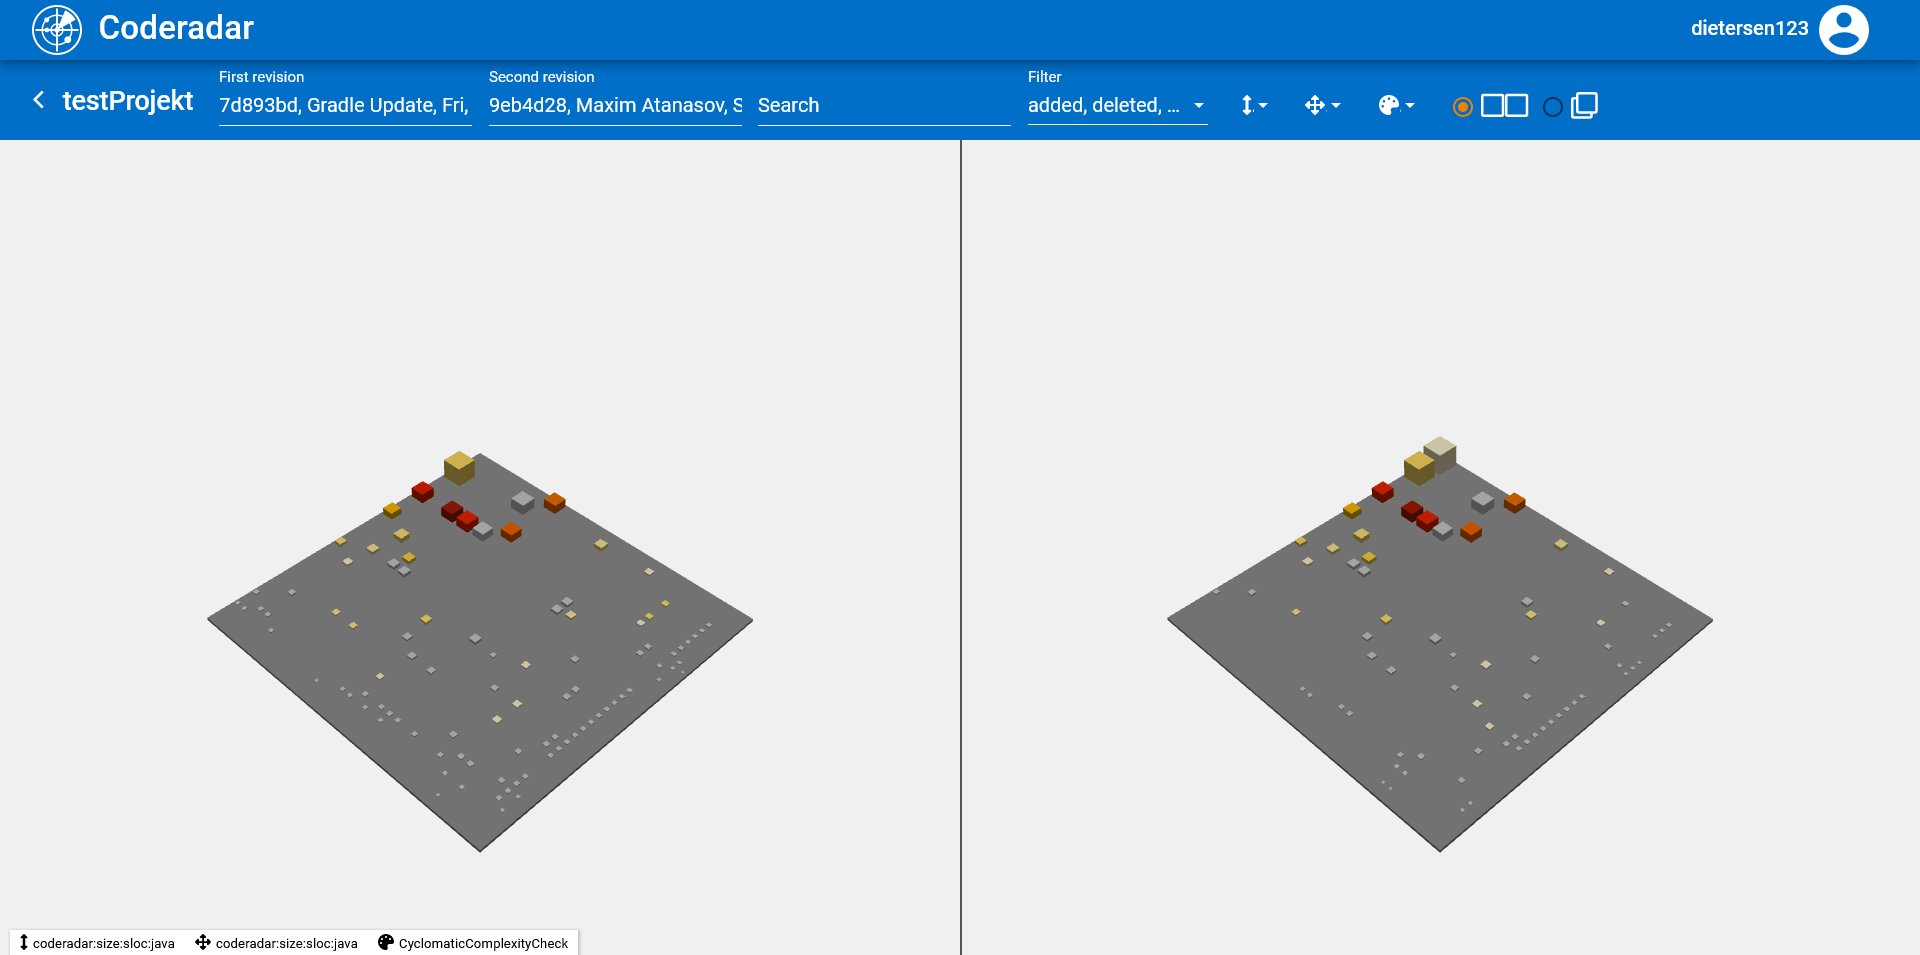
\includegraphics[width=\linewidth]{images/city_view}
		\caption{Ein Beispiel für die City-View.}
		\label{city_view}
	\end{center}
\end{figure}

\begin{figure}[htb]
	\begin{center}
		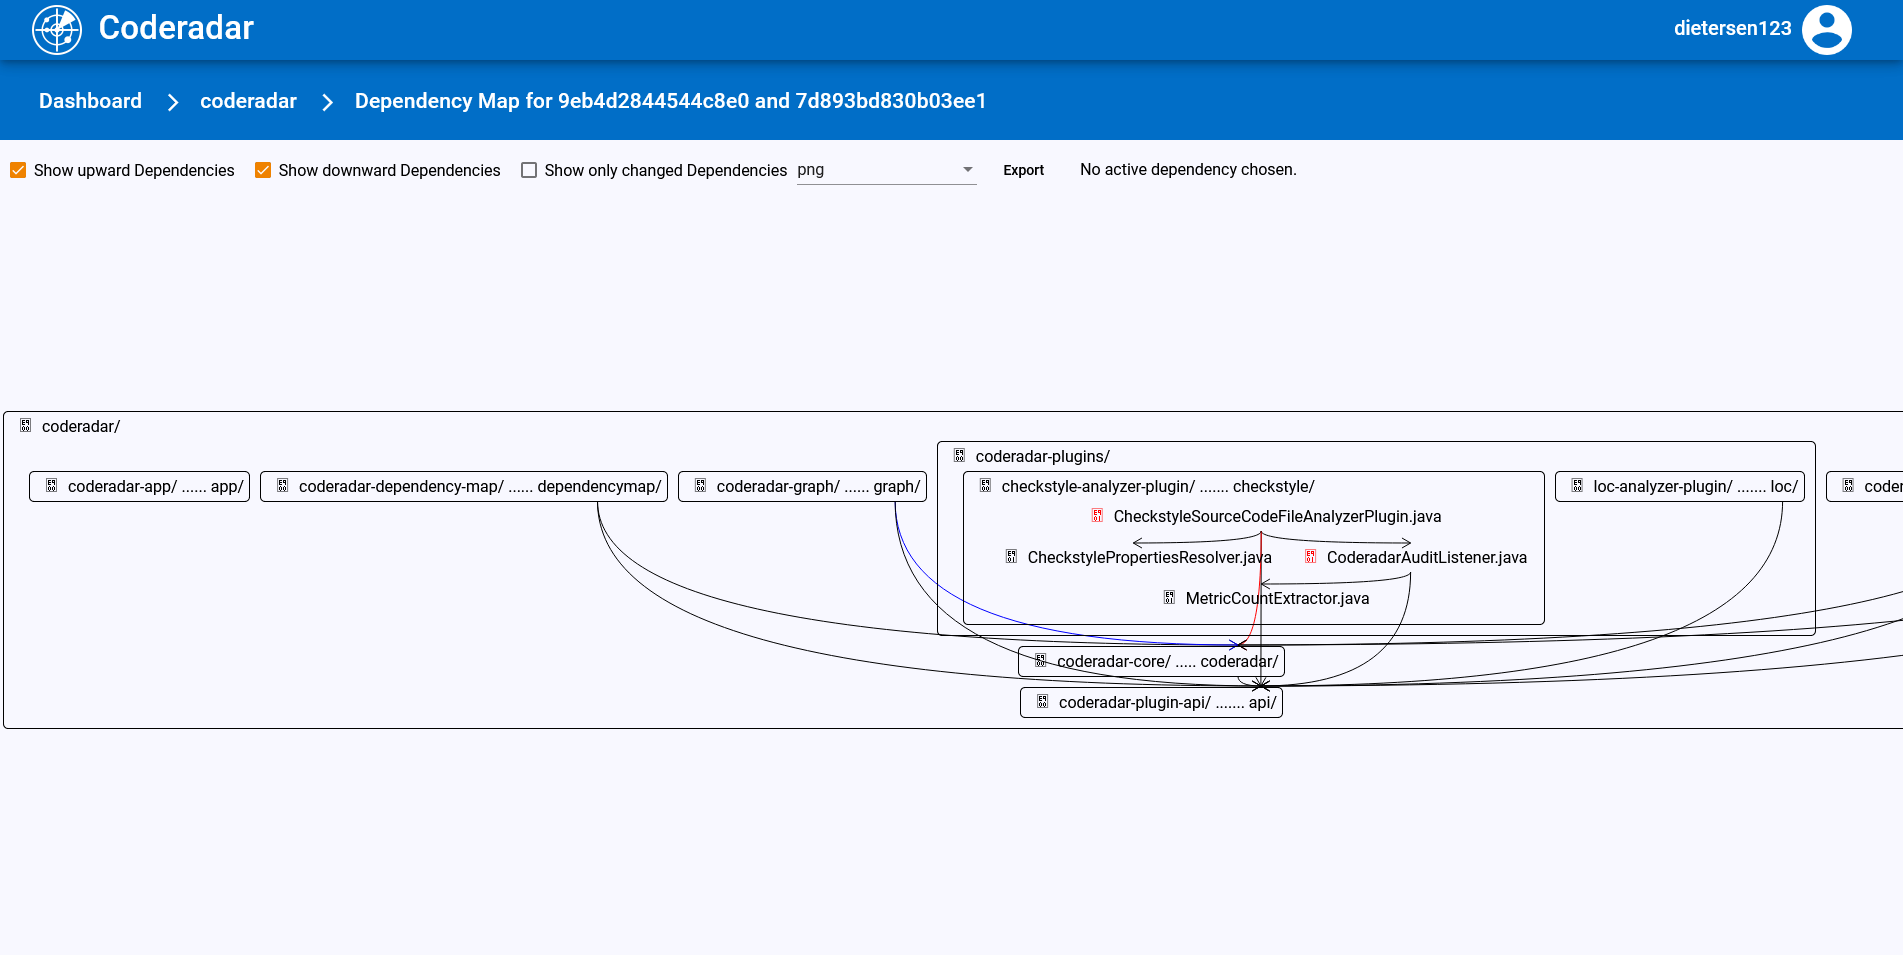
\includegraphics[width=\linewidth]{images/dependency_map}
		\caption{Ein Beispiel für die Dependency-Map.}
		\label{dependency_map}
	\end{center}
\end{figure}

\begin{figure}[htb]
	\begin{center}
		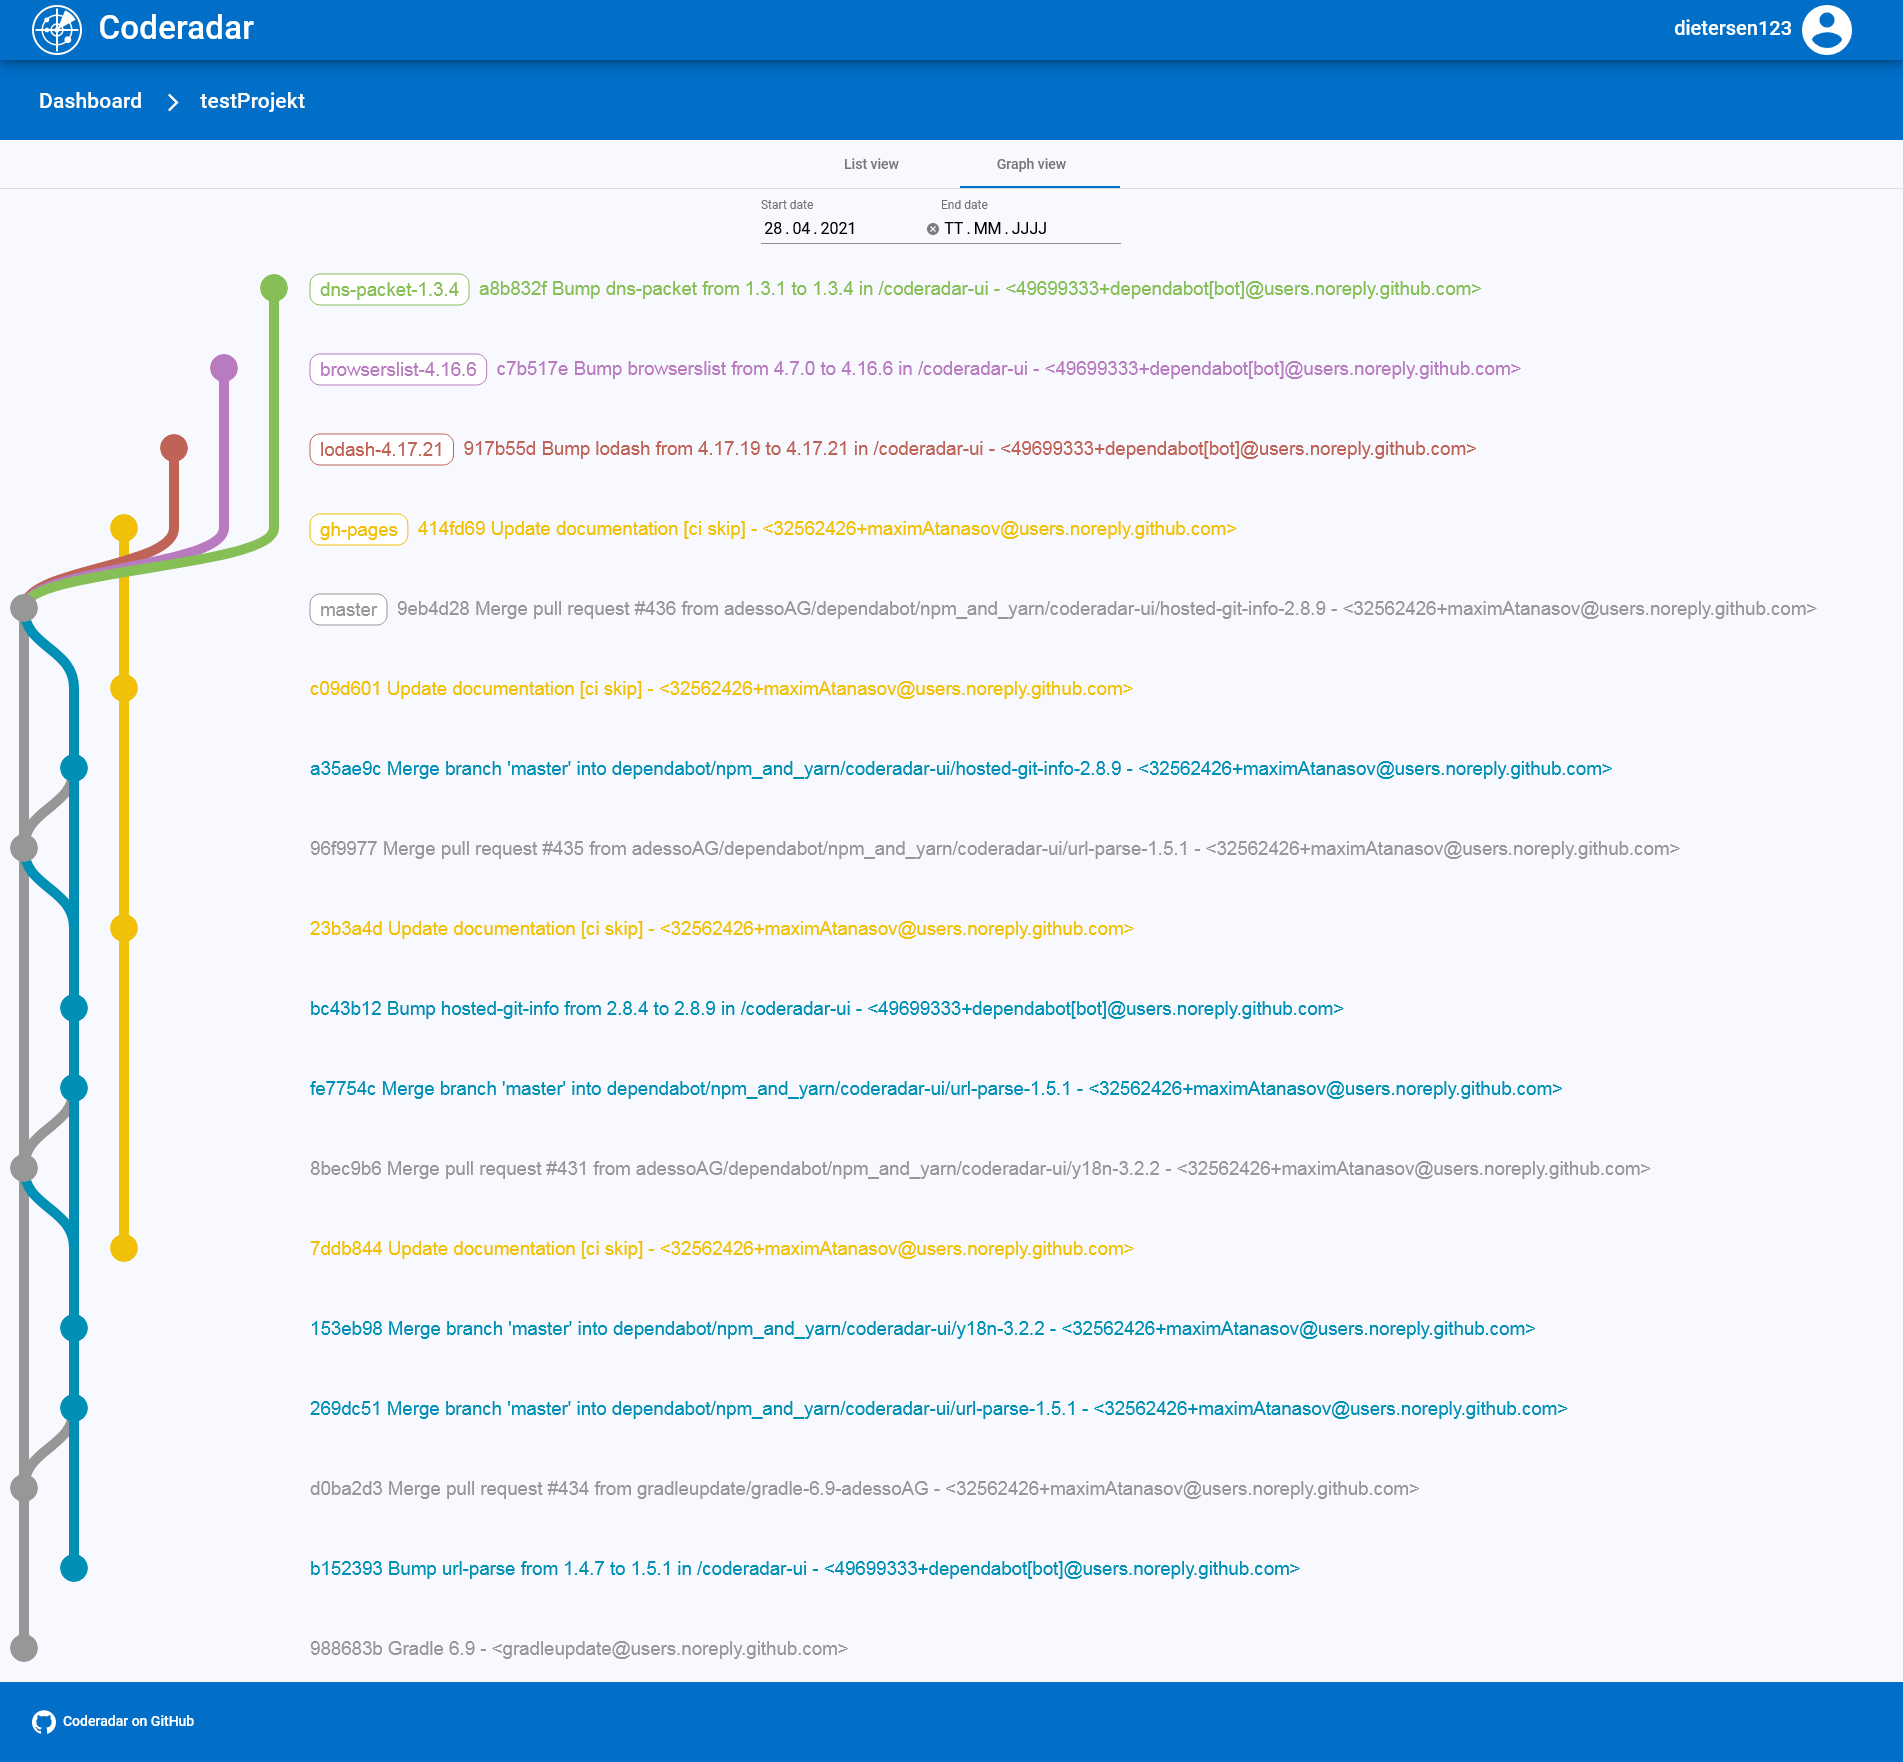
\includegraphics[width=\linewidth]{images/tree_view}
		\caption{Die Baumansicht der Commits in coderadar.}
		\label{tree_view}
	\end{center}
\end{figure}

%___________________________________________________________________________________________________

% Abkürzungsverzeichnis ins Inhaltsverzeichnis aufnehmen und mit Inhalt füllen
\cleardoublepage\phantomsection\addcontentsline{toc}{chapter}{Abkürzungsverzeichnis}
\chapter*{Abkürzungsverzeichnis}
\begin{acronym}
	\acro{REST}{Representational State Transfer} % 439
	\acro{SOAP}{Simple Object Access Protocol} % 439
	\acro{OWASP}{Open Web Application Security Project} % 480
	\acro{CWE}{Common Weakness Enumeration} % 572
	\acro{CLI}{Command Line Interface} % 685		
	\acro{JRE}{Java Runtime Environment} % 706
	\acro{LOC}{Lines of Code} % 769
\end{acronym}

\newpage{}

% Weitere Verzeichnisse ins Inhaltsverzeichnis aufnehmen
\cleardoublepage\phantomsection\addcontentsline{toc}{chapter}{Abbildungsverzeichnis}
\listoffigures

\newpage{}

\cleardoublepage\phantomsection\addcontentsline{toc}{chapter}{Tabellenverzeichnis}
\listoftables

\lstlistoflistings 
	
% Literaturverzeichnis setzen
\bibliographystyle{alphadin}
\bibliography{bib}
	
% Eidesstattliche Erklärung. ACHTUNG: Korrekten Text bitte unbedingt vorab mit Studienbüro klären!
\chapter*{Eidesstattliche Erklärung}
\thispagestyle{empty}
\textbf{ACHTUNG: Korrekten Text bitte unbedingt vorab mit Studienbüro klären!}\\
Hiermit versichere ich gemäß § 18 Abs. 5 der Bachelor-Prüfungsordnung des Studiengangs Informatik aus dem Jahr 2013, dass ich die  vorliegende Arbeit selbstständig angefertigt und mich keiner fremden Hilfe bedient, sowie keine anderen als die angegebenen Quellen und Hilfsmittel benutzt habe. Alle Stellen, die wörtlich oder sinngemäß veröffentlichten oder nicht veröffentlichten Schriften und anderen Quellen entnommen sind, habe ich als solche kenntlich gemacht. Diese Arbeit hat in gleicher oder ähnlicher Form noch keiner Prüfungsbehörde vorgelegen.

\vspace{1\baselineskip}%
Dortmund, \fhdopaperdate \hfill \fhdopaperauthor
\end{document}